\label{chapter:reflection}

In Chapter~\ref{chapter:structsens}, we targeted the problem of lost
structural information in C/C++ programs by employing a pointer
analysis that recovers lost memory structure via a variety of
techniques. In this chapter and the next, we shift our focus to Java:
a higher-level strongly-typed language with no capabilities for direct
memory access.
%
Still, essential structural information is often lost in Java programs
too, yet for different reasons. As stated in
Chapter~\ref{chapter:intro}, a source of analysis imprecision,
especially in determining the types of abstract objects constructed by
the analysis, lies in the usage of Java's reflection mechanism: the
ability to inspect and dynamically retrieve classes, methods, attributes,
etc. at runtime.

By using the Reflection API, Java programs can encompass dynamic
behavior. However, statically reasoning about the behavior of software
that uses reflection can be especially cumbersome.
%
Unfortunately, reflection is ubiquitous in large Java programs.
% static reflection handling is hard because of the ubiquity of reflection in real
% programs and because of the size of Java programs and libraries.
%
Any handling of reflection will be approximate, and overestimating its
reach in a large codebase can be catastrophic for precision and
scalability. In this chapter, we present an approach for handling
reflection with improved empirical soundness (as measured against
prior approaches and dynamic information), again, in the context of a
points-to analysis. Our approach is based on the combination of
string-flow and points-to analysis from past literature augmented with
\begin{inparaenum}[(a)]
\item substring analysis and modeling of partial string flow through
  string builder classes;
\item new techniques for analyzing reflective entities based on
  information available at their use-sites (similar to those presented
  in Chapter~\ref{chapter:structsens}).
\end{inparaenum}
% The resulting analysis is general, without any need for hand-tuning. 
In experimental comparisons with prior approaches, we demonstrate a
combination of both improved soundness (recovering the majority of
missing call-graph edges) and increased performance.

% achieves near-complete coverage of the target program: our static
% heuristics seem to truly offer an over-approximation of dynamic
% behavior, without sacrificing scalability. Whereas past studies have
% shown hundreds of methods (as much as 40\% of the dynamically
% reachable methods) to be statically undiscovered, we achieve over 97\%
% completeness at virtually no extra cost.

\section{Intro: Static Analysis and Java Reflection}

Whole-program static analysis is the engine behind several modern
programming facilities for program development and
understanding. Compilers, bug detectors, security checkers, modern
development environments (with automated refactorings, slicing
facilities, and auto-complete functionality), and a myriad other tools
routinely employ static analysis machinery. Even the seemingly simple
effort of computing a program's call-graph (i.e., which program
function can call which other) requires sophisticated analysis in
order to achieve precision in a modern language.

Yet, static whole-program analysis suffers in the presence of common
dynamic features, especially reflection. When a Java program accesses
a class by supplying its name as a run-time string, via the
\javasignature{Class.forName} library call, the static analysis has
very few available courses of action: It needs to either
conservatively over-approximate (e.g., assume that \emph{any} class
can be accessed, possibly limiting the set later, after the returned
object is used), or to perform a string analysis that will allow it to
infer the contents of the \code{forName} string argument. Both options
can be detrimental to the scalability of the analysis: the
conservative over-approximation may never become constrained enough by
further instructions to be feasible in practice; precise string
analysis is impractical for programs of realistic size.  It is telling
that \emph{no practical Java program analysis framework in existence
  handles reflection soundly} \cite{soundiness15}, although other
language features are modeled soundly.\footnote{In our context,
  \emph{sound} = over-approximate, i.e., guaranteeing that all
  possible behaviors of reflection operations are modeled.}

%
Full soundness is not practically achievable, but it can still be
approximated for the well-behaved reflection patterns encountered in
regular, non-adversarial programs.  Therefore, it makes sense to treat
soundness as a continuous quantity: something to improve on, even
though we cannot perfectly reach.  To avoid confusion, we use the term
\emph{empirical soundness} for the quantification of how much of the
dynamic behavior the static analysis covers. Computable metrics of
empirical soundness can help quantify how close an analysis is to the
fully sound result. Based on such metrics, one can make comparisons
(e.g., ``more sound'') to describe soundness improvements.

%An analysis is termed ``soundy'', when it is ``sound modulo
%well-known sources of unsoundness'', such as
%reflection \cite{soundiness15}.

%Empirical soundness is the quantification of the gap between soundy and
%(the unattainable) fully sound. The techniques presented in this
%chapter serve as a step in that direction: beyond soundy, yet not fully
%sound.


%After all, the reason to perform static
%analysis is to capture more program behaviors than a dynamic
%execution---the converse is a paradox that puts the value of the
%static analysis in question. Even if guaranteed full soundness is
%impractical, it is desirable to capture most actual behavior for the
%well-behaved reflection patterns encountered in regular,
%non-adversarial programs.

The second challenge of handling reflection in a static analysis is
\emph{scalability}.  The online documentation of the IBM \textsc{Wala}
library~\cite{www:wala-reflection} concisely summarizes the current
state of the practice, for \emph{points-to analysis} in the Java
setting.

\begin{quote}
  \emph{Reflection usage and the size of modern libraries/frameworks
    make it very difficult to scale flow-insensitive points-to
    analysis to modern Java programs. For example, with default
    settings, \textsc{Wala}'s pointer analyses cannot handle any
    program linked against the Java 6 standard libraries, due to
    extensive reflection in the libraries.}
\end{quote}

\noindent The same caveats routinely appear in the research
literature. Multiple published points-to analysis papers analyze
well-known benchmarks with reflection
disabled~\cite{popl/SmaragdakisBL11,pldi/KastrinisS13,ecoop/AliL12,ecoop/AliL13}.


A representative quote~\cite{popl/SmaragdakisBL11} illustrates:
\begin{quote}
  \emph{Hsqldb and jython could not be analyzed with reflection
    analysis enabled [...]  ---hsqldb cannot even be analyzed
    context-insensitively and jython cannot even be analyzed with the
    1obj analysis. This is due to vast imprecision introduced when
    reflection methods are not filtered in any way by constant strings
    (for classes, fields, or methods) and the analysis infers a large
    number of reflection objects to flow to several variables.  [...]
    For these two applications, our analysis has reflection reasoning
    disabled.  Since hsqldb in the DaCapo benchmark code has its main
    functionality called via reflection, we had to configure its entry
    point manually.}
\end{quote}

%\noindent
In this chapter, we describe an approach to analyzing reflection in the
Java points-to analysis setting.
%Points-to analysis consists
%of computing which objects (abstracted as allocation sites) a program
%variable can reference. The analysis is the backbone of many realistic
%static analyses, as it offers a scalable way to model heap behavior.
%
%Notably, both of the
%above quotes regarding the difficulties of reflection handling are in
%the context of points-to analyses.
%
Our approach requires no manual configuration and achieves
significantly higher empirical soundness without sacrificing
scalability, for realistic benchmarks and libraries (DaCapo Bach and
Java 7).
%% than those that past work failed to analyze.
% As we shall see, our analysis implements (and
%enables to run with full reflection support) the same points-to
%algorithms that in the past could not scale to some benchmarks, all
%using the Java 6 standard libraries, which the \textsc{Wala} documentation
%warns about. 
%
%There are two new technical elements in our work:
%
%\begin{bullets}
%\item We augment prior algorithms for inter-related reflection and
%points-to analysis \cite{aplas/LivshitsWL05,livshits:thesis} with a
%\emph{substring} analysis, as well as a string flow analysis.  
%%
%%While
%%past approaches have required user specifications to determine the
%%possible target of reflective calls whose input was partially dynamic,
%%we attempt to over-approximate without sacrificing scalability. For
%%instance, consider the case of a program that contains a constant
%%string, \code{"Handler"}, which partially matches reflection-accessible
%%entities of the program code---e.g., a class name
%%``\code{somePackage.EventHandler}'', or a method name
%%``\code{callbackHandler}''. If our string flow analysis determines that
%%this string flows (through standard Java API string operators such as
%%\code{+}, which resolves to \code{append} and \code{toString}) to the site
%%of a \code{forName} call, it will conservatively assume that the
%%reflection object (aka ``class object'') for class
%%\code{somePackage.EventHandler} can be returned at that
%%point. Similarly, if the \code{"Handler"} string (however augmented by
%%concatenations) flows to the site of a reflective call (such as
%%\javasignature{Class.getMethod}) that attempts to retrieve a method from a class
%%object containing method \code{callbackHandler}, the analysis will
%%compute that the call may return the reflection object for this
%%method.
%%
%The insight behind this treatment is that reflection is often used to
%dynamically access entities with partially known names, and the
%dynamic part of the configuration is limited to package prefixes,
%method name suffixes, etc. Thus, much of the dynamic information
%(i.e., other substrings contributing to the eventual string
%representing a class or member name) can be supplanted by
%mere over-approximation.
%
%
%%The merging
%%of string constants is a very common optimization technique that
%%significantly improves performance (TODO: citation needed).
%
%\item We introduce new techniques for inferring the result of
%  reflection calls based on how this result is used later in the
%  program. Consider, for instance, a sequence of program statements,
%  possibly remote to each other, yet with values flowing from one to
%  the next:
%
%\begin{code}
%\begin{small}
%\begin{verbatim}
%Class c1 = Class.forName(className);
%...      // c2 aliases c1
%Object o1 = c2.newInstance(); 
%...      // o2 aliases o1
%e = (Event) o2; 
%\end{verbatim}
%\end{small}
%\end{code}
%
%%String className = ... ;
%%
%%Object o = c.newInstance();
%%String methodName = ... ;
%%Method m = c.getMethod(methodName, ...);
%%m.invoke(o, ...);
%
%%If we know that the object held by \code{o} is the result of a reflection
%%operation (e.g., the return value of a \javasignature{Field.get} or a
%%\javasignature{Method.invoke} call) then we immediately get information on the
%%reflection call that produced \code{o}, by assuming that the cast is
%%intended to succeed. 
%
%Assuming that the cast is intended to succeed, we get information
%regarding the result of the \code{newInstance} call, which, in turn,
%informs the result of the \code{forName} call. That is, by keeping track
%of the flow of objects from an original call that accepts strings and
%produces reflection objects (such as a \code{forName} or a \code{getField}
%call) we infer that this string could have been the
%name of a subtype of \code{Event}. This effectively propagates
%information back to the source of an unknown object.
%
%Similar reasoning has been employed in other work
%\cite{aplas/LivshitsWL05,ecoop/LiTSX14}. Yet our approach generalizes
%past techniques significantly: we support patterns such as the above
%inter-procedurally and in full generality, leverage information from
%strings and not just casts, and introduce ``invented'' objects that
%materialize at the point of a cast and subsequently aid the analysis
%modeling.
%
%
%%%%SPACE (probably not only)
%% Our approach has three
%%differences.  First, our analysis is completely inter-procedural: we
%%allow the last two statements of the above example to occur in distant
%%methods, and leverage the base points-to analysis to track object
%%flow.  In contrast, all past techniques required  the cast
%%operation not only to be in the same method as the \code{newInstance}
%%(or other similarly treated calls) but also to post-dominate
%%it. Second, we leverage use-based information from strings, and not
%%just from casts. For instance, a \javasignature{Class.getMethod} or
%%\javasignature{Class.getField} call with a constant string parameter gives
%%information that can narrow down what the receiver \code{Class} object
%%may be. Lastly, we introduce ``invented'' objects that fully
%%materialize at the point of a cast and participate in the analysis
%%afterwards. In our example, if a special marker object is found to
%%flow to variable \code{o2} from a reflection call, in addition to
%%propagating information back to the reflection call, a new
%%invented object of type \code{Event} will be considered to exist
%%at the point of the cast, to represent all objects possibly missed. By
%%carefully balancing the amount of information propagated back to the
%%reflection call vs. the new objects invented at cast points, we trade
%%off scalability for soundness. For instance, if a cast does not
%%significantly narrow down the possible \code{Class} objects returned by
%%a distant \code{forName} call, we do not propagate information backwards
%%to the \code{forName} call site, as this would be detrimental to
%%precision and scalability. (The site would appear to create a many
%%different \code{Class} objects, which will propagate down and pollute
%%all intermediate reflective calls.)  Instead, in this case we will
%%only propagate an invented object forward.
%%
%%\end{bullets}
%%
%% ideas
%%that were earlier only applied intra-procedurally; it infers objects
%%based on string constants; and it creates usable abstract
%%representations of objects it cannot identify (whereas past work only
%%treated such objects as placeholders).
%
%\item We carefully tune the context-sensitivity and object
%  discrimination policies of our analysis to maintain scalability, by
%  avoiding an explosion in the number of entities. For instance, we
%  remove context-sensitivity from reflective method invocations and
%  object creation, although context-sensitivity is restored for
%  methods called directly (i.e., virtual or static calls) inside
%  reflectively called methods. Similarly, we merge the points-to
%  handling of all string objects representing method or field names
%  (but not class names), while still remembering (over-approximately)
%  which reflection entities they may refer to. Additionally, we merge
%  string factory objects (instances of library classes
%  \code{StringBuilder} or \code{StringBuffer}) despite the need to track
%  substring flow through them. Essentially, if a substring whose name
%  may refer to a reflection entity $E$ flows to \emph{any} string
%  factory, and \emph{any} string factory feeds into a reflective call,
%  reflection entity $E$ is inferred to possibly be the result of the
%  call. Intuitively, the above broad over-approximation does not affect
%  much the precision of our approach because the enabling conditions
%  provide a good filter and because precision is often restored in
%  practice when the code casts the result of a reflective call to a
%  certain type.
%
%We apply our approach to the \textsc{Doop} framework~\cite{oopsla/BravenboerS09} and
%evaluate it using the DaCapo benchmarks. We find that our techniques
%achieve very high empirical soundness, as measured in call-graph edges
%relative to
%%(several) 
%dynamic executions. For comparison, the earlier reflection treatment
%of \textsc{Doop}, which implemented the algorithm of Livshits et
%al.~\cite{aplas/LivshitsWL05},
%% without any of our enhancements, 
%missed many tens to hundreds of call-graph edges for each benchmark
%\cite{ecoop/AliL12,ecoop/AliL13} and even required
%manual configuration to achieve this result. Furthermore, we make no
%sacrifices in scalability: our analyses scale just as well as (or
%better than) the original \textsc{Doop} analyses even for modern large JDKs.
%
%As a result of carefully balancing the soundness and scalability of
%all techniques, our approach is more sound than past work, without
%sacrificing scalability. 
%
In experimental comparisons with the recent \textsc{Elf}
system~\cite{ecoop/LiTSX14} (itself improving over the reflection
analysis of the \textsc{Doop} framework~\cite{oopsla/BravenboerS09}),
our algorithm discovers most of the call-graph edges missing (relative
to a dynamic analysis) from \textsc{Elf}'s reflection analysis.  This
improvement in empirical soundness is accompanied by \emph{increased}
performance relative to \textsc{Elf}, demonstrating that near-sound
handling of reflection is often practically possible. Concretely, our
work:
\begin{itemize}[\(\cdot\)]
%\item offers the first static handling of Java reflection that 
% exhibits both high empirical soundness and performance for
% sophisticated analyses and large-scale benchmarks, with no
% extra inputs;
\item introduces key techniques in static reflection handling that
  contribute greatly to empirical soundness. The techniques generalize
  past work from an intra-procedural to an inter-procedural setting
  and combine it with a string analysis;
\item shows how scalability can be addressed with appropriate tuning
  of the above generalized techniques;
\item thoroughly quantifies the empirical soundness of a static
  points-to analysis, compared to past approaches and to a dynamic
  analysis;
\item is implemented and evaluated on top of an existing open
  framework (\textsc{Doop}~\cite{oopsla/BravenboerS09}).
  % This can offer a platform for experimentation with sophisticated
  % static reflection handling, possibly also leading to good static
  % handling of other dynamic features (e.g., complex dynamic
  % loading).
\end{itemize}

%%%SPACE
%The rest of the chapter introduces important background on static
%reflection analysis (Section~\ref{reflection/sec:model}), presents our new
%techniques (Section~\ref{reflection/soundiness}), evaluates them
%(Section~\ref{reflection/sec:experiments}), and compares to related work
%(Section~\ref{reflection/sec:related}).


\section{Points-to Analysis in Java}
\label{reflection/sec:javapt}

In Chapter~\ref{chapter:structsens}, we presented a points-to analysis
for C/C++ that includes various enhancements to make it
structure-sensitive. Before presenting our enhancements towards better
handling of Java's reflection, we first present a typical points-to
analysis for Java and discuss its fundamental differences from
analyzing C/C++.

The domains of the analysis include:
\begin{compactitem}[\(\cdot\)]
\item variables, \(V\)
\item (class) types, \(T\)
\item fields, \(F\)
\item methods, \(M\)
\item abstract (heap) objects, \(H\)
\item instruction labels, \(L\)
\item and strings.
\end{compactitem}

\begin{figure}[t]
  \centering
  \begin{tabular}{l@{\quad}l@{\qquad}l}
    \toprule
    \emph{Java Instruction}
    & \emph{Operand Types}
    & \emph{Description} \\
    \midrule
    \(\newinstr{p}{C}\)
    & \(V \!\times\! T\)
    & Heap Allocations
    \\
    \(\castinstr{p}{T}{q}\)
    & \(V \!\times\! T \!\times\! V\)
    & Casts
    \\
    \(\moveinstr{p}{q}\)
    & \(V \!\times\! V\)
    & Assignments
    \\
    \(\fldloadinstr{p}{q}{f}\)
    & \(V \!\times\! V \!\times\! F\)
    & Field Loads
    \\
    \(\fldstoreinstr{p}{f}{q}\)
    & \(V \!\times\! F \!\times\! V\)
    & Field Stores
    \\
    \(\vcallinstr{p}{v}{meth}\)
    & \(V \!\times\! V \!\times\! M \!\times\! V^n\)
    & Virtual Calls
    \\
    \(\scallinstr{p}{C}{meth}\)
    & \(V \!\times\! T \!\times\! M \!\times\! V^n\)
    & Static Calls
    \\
    \(\returninstr{p}\)
    & \(V\)
    & Method Returns
    \\
    \bottomrule
  \end{tabular}
  \caption[Java Instruction Set]{%
    Java Instruction Set. We also prepend a label $l \in L$ to each
    instruction (that we omit in this figure). Each such label can be
    used to uniquely identify its instruction. %
  }
  \label{structsens/fig/javair}
\end{figure}

Figure~\ref{structsens/fig/javair} lists the basic Java instructions,
relevant to a points-to analysis. We note some key differences from
the C/C++ setting:
\begin{itemize}[--]
\setlength\itemsep{0.3em}
\item there are no pointer types, or any way to directly operate on
  memory addresses
\item there is a clear distinction between variables (allocated on the
  stack) and objects (allocated on the heap)
\item loads and stores need a field operand
\item there are two types of method call instructions:
  \begin{inparaenum}[(i)]
  \item virtual calls (that perform dynamic dispatch based on the
    dynamic type of the receiver), and
  \item static calls.
  \end{inparaenum}
\end{itemize}

\begin{figure}[h!t]
  \begin{math}
    \inferrule* [left=Alloc\,]
    {\newinstr[i]{p}{T}}
    {\vpt{p}{o_{i}}
      \\ \alloctype{o_{i}} = \tp{T}}
  \end{math}
  \\

  \begin{math}
    \inferrule* [left=Cast\,]
    {\castinstr[i]{p}{T}{q}
      \\ \vpt{q}{o_{i}}
      \\ \alloctype{o_{i}} = \tp{T'}
      \\ \subtypeof{T'}{T}}
    {\vpt{p}{o_{i}}}
  \end{math}
  \\

  \begin{math}
    \inferrule* [left=Move\,]
    {\moveinstr[i]{p}{q}
      \\ \vpt{q}{o_{i}}}
    {\vpt{p}{o_{i}}}
  \end{math}
  \\

  \begin{math}
    \inferrule* [left=Load\;]
    {\fldloadinstr[i]{p}{q}{f}
      \\ \vpt{q}{o_b}
      \\ \fieldpt{o_b}{f}{o}}
    {\vpt{p}{o}}
  \end{math}
  \\

  \begin{math}
    \inferrule* [left=Store\;]
    {\fldstoreinstr[i]{p}{f}{q}
      \\ \vpt{p}{o_b}
      \\ \vpt{q}{o}}
    {\fieldpt{o_b}{f}{o}}
  \end{math}
  \\

  \begin{math}
    \inferrule* [left=VCall\;]
    {\vcallinstr[i]{p}{v}{meth}
      \\ \vpt{v}{o}
      \\ \alloctype{o} = \tp{T}
      \\ \lookup{T}{meth} = \code{meth}\rq}
    {i \xrightarrow{calls} \code{meth}\rq\,(\ldots)
      \\ \vpt{this\(_{\,\code{meth}\rq}\)}{o}}
  \end{math}
  \\

  \begin{math}
    \inferrule* [left=SCall\;]
    {\scallinstr[i]{p}{C}{meth}}
    {i \xrightarrow{calls} \tp{C}\,.\,\code{meth}\,(\ldots)}
  \end{math}
  \\

  \begin{math}
    \inferrule* [left=Args\;]
    {\callinstr[i]{p}{x\,.\,\code{meth}}[\var{a}_1][\var{a}_2,\ldots,\var{a}_n]
      \\ i \xrightarrow{calls} \code{meth}\rq\,(\var{v}_1,\, \var{v}_2,\, \ldots,\,\var{v}_n)}
    {\forall j:\ \opt{\var{a}_j}{o} \;\Rightarrow\; \opt{\var{v}_j}{o}}
  \end{math}
  \\

  \begin{math}
    \inferrule* [left=Ret\;]
    {\callinstr[i]{p}{x\,.\,\code{meth}}
      \\ i \xrightarrow{calls} \code{meth}\rq\,(\ldots)
      \\ \returninstr[j]{q}
      \\ j \in \body{\code{meth}\rq}
      \\\\ \vpt{q}{o}}
    {\vpt{p}{o}}
  \end{math}
  \caption{Inference Rules for Java Points-to Analysis}
  \label{reflection/fig/javapointsto}
\end{figure}

Figure~\ref{reflection/fig/javapointsto} presents a standard Java
points-to analysis
\cite{uss/GuarnieriL09,pldi/KastrinisS13,aplas/WhaleyACL05}, expressed
in inference rules (as those of Chapter~\ref{chapter:structsens}). The
basic relations it computes are:
\begin{description}
\item[Variable points-to edges.] Edge \(\vpt{v}{o} \in V \times H\)
  records that variable \var{v} may point to abstract object
  \(\alloc{o}\).
\item[Field points-to edges.] Edge
  \(\fieldpt{o_b}{fld}{o} \in H \times F \times H\) records that
  abstract object \(\alloc{o_b}\) may point to abstract object
  \(\alloc{o}\), via field \(\code{fld}\). Field points-to edges can
  only be established by field store instructions.
\item[Abstract object types.] The partial function
  \(\typefunc: H \nrightarrow T\) records the type of an abstract
  object. Reflection aside, each abstract object will be associated
  with a single type that will be readily available at the allocation
  site.
\item[Call-graph edges.] Edge
  \(i \xrightarrow{calls} m \in L \times M\) records that invocation
  site \(i\) may call method \(m\) (after the dynamic dispatch has
  been resolved).
\end{description}

Note that, without reflection, a points-to analysis needs only create
a single kind of abstract objects that represents heap allocations
based on the allocation site. There is no need for abstract
subobjects, since
\begin{inparaenum}[(i)]
\item heap objects can only contain references to other objects but
  cannot embed the actual allocations; complex structures need to be
  dispersed through the heap and accessed via multiple field loads
\item a variable can only point to the start of a heap allocation.
\end{inparaenum}
However, more types of abstract objects that serve our
reflection-related enhancements will be introduced later.

The first rule of Figure~\ref{reflection/fig/javapointsto} creates a
typed abstract object that represents the given allocation site, and
assigns it to the target variable. The next two rules, handling cast
and move instructions, simply copy the points-to set of the source to
that of the target variable. For cast instructions, however, we also
perform a type check to filter objects of incompatible types (by
checking if the type of the allocation is a subtype of the type of the
variable). Since Java is strongly-typed, this is the only place
where we can benefit from such a type check; any other points-to edges
established by the rest of the rules are guaranteed to be
type-compatible.

The next two rules handle load and store instructions. To load from a
field, we have to follow the relevant field points-to edge of any base
object that we may load from. Inversely, storing to a field
establishes such field points-to edges between any heap objects that
the base and source variable may point to.

For virtual calls, we first have to determine the type(s) of the
receiver object(s), and determine the actual method that will be
called after method resolution. (For this purpose, we assume the
existence of a \emph{lookup} function that performs the actual
resolution.) Then, we can establish a call-graph edge for the given
allocation site, as well as a points-to edge for variable \code{this}
of the resolved method. Static calls are simpler, since they require
no method resolution and have no receivers. The last two rules apply
to both virtual and static calls, and model call and return
instructions as (interprocedural) assignments (similarly to the C/C++
setting), regarding method arguments and returned values.


\section{Joint Reflection and Points-To Analysis}
\label{reflection/sec:model}

Next, we extend our abstracted model of the points-to analysis with
an inter-related reflection analysis.
%
The model is a light reformulation of the analysis introduced by Livshits et
al.~\cite{aplas/LivshitsWL05,livshits:thesis}.  The main insight of
the Livshits et al. approach is that reflection analysis relies on
points-to information, because the different key elements of a
reflective activity may be dispersed throughout the program. A typical
pattern of reflection usage is with code such as:

\begin{javacodelinum}
String className = ... ;
Class c = Class.forName(className);
Object o = c.newInstance();
String methodName = ... ;
Method m = c.getMethod(methodName, ...);
m.invoke(o, ...);
\end{javacodelinum}

All of the above statements can occur in distant program locations,
across different methods, invoked through virtual calls from multiple
sites, etc. Thus, a whole-program analysis with an understanding of
heap objects is required to track reflection with any amount of
precision. This suggest the idea that reflection analysis can leverage
points-to analysis---it is a client for points-to information. At the
same time, points-to analysis needs the results of reflection
analysis---e.g., to determine which method gets invoked in the last
line of the above example, or what objects each of the example's local
variables point to. Thus, under the Livshits et al. approach,
reflection analysis and points-to analysis become mutually recursive,
or effectively a single analysis.

Recall that, in the C/C++ setting of Chapter~\ref{chapter:structsens},
we used the same insight to associate untyped abstract objects with
their possible types. The points-to analysis is used as both a
producer and consumer of type information: new type-object
associations drive the creation of new abstract objects, altering the
points-to results that may, again, produce new type information, and so
on.

% Such mutual recursion introduces significant complexity.  Fortunately,
% a large amount of research in points-to analysis has focused on
% specifying analyses declaratively
% \cite{repsdb,aplas/WhaleyACL05,pods/LamWLMACU05,pldi/WhaleyL04,oopsla/BravenboerS09,cc/KastrinisS13,issta/BravenboerS09,pldi/KastrinisS13,pldi/NaikAW06,pldi/LiangN11,uss/GuarnieriL09},
% in the Datalog programming language. Datalog is ideal for encoding
% mutually recursive logic---recursion is the backbone of the
% language. Computation in Datalog consists of monotonic logical
% inferences that apply to produce more facts until fixpoint. A Datalog
% rule ``\pred{C}{z,x} \rulearrow{} \pred{A}{x,y}, \pred{B}{y,z}.''
% means that if \pred{A}{x,y} and \pred{B}{y,z} are both true, then
% \pred{C}{z,x} can be inferred. Livshits et al. expressed their joint
% reflection and points-to analysis declaratively in Datalog, which is
% also a good vehicle for our illustration and further changes.

We consider the core of the analysis algorithm, which is
representative and handles the most common features, illustrated in
our above example: creating a reflective object representing a class
(a \emph{class object}) given a name string (library method
\javasignature{Class.forName}), creating a new object given a class
object (library method \javasignature{Class.newInstance}), retrieving
a reflective method object given a class object and a signature
(library method \javasignature{Class.getMethod}), and reflectively
calling a virtual method on an object (library method
\javasignature{Method.invoke}). This treatment ignores several other
APIs, which are handled similarly. These include, for instance,
fields, constructors, other kinds of method invocations (static,
special), reflective access to arrays, other ways to get class
objects, and more.

The Livshits et al. reflection analysis can be expressed as a
four-rule addition to the points-to analysis of
Section~\ref{reflection/sec:javapt}. However, we first have to extend
our domain of abstract heap objects with some special kinds of
\emph{reflective objects}. These new kinds of objects consist of the
following:

\begin{minipage}{\linewidth}
  \renewcommand{\arraystretch}{1.5}
  \begin{tabular}{@{--\ }l@{\quad}p{0.87\textwidth}}
    \(\alloc{\reifiedclass{T}}\)
    & Represents the reflective class object for class type \(\tp{T} \in T\).
    \\[3pt]
    \(\alloc{\reifiedmethod{m}}\)
    & Represents the reflective object for method \(\code{m} \in M\).
    \\[3pt]
    \(o_{i,\tp{T}}\)
    & Represents objects of type \(\tp{T} \in T\) that are allocated with a
      \code{newInstance()} call at invocation site \(i \in L\).
    \\
  \end{tabular}
\end{minipage}

% The analysis takes as input the relations (i.e., tables filled with
% information from the program text) shown in
% Figure~\ref{reflection/figure:inputs}.  Using these inputs, the
% Livshits et al. reflection analysis can be expressed as a five-rule
% addition to any points-to analysis.
% The rest of the points-to analysis (not shown here---see e.g.,
% \cite{uss/GuarnieriL09,pldi/KastrinisS13,aplas/WhaleyACL05}) supplies
% more rules for computing a relation \pred{VarPointsTo}{v: V, h: H} and
% a relation \pred{CallGraphEdge}{i: I, m: M}.
% % TODO put in chapter summary
% Intuitively, the traditional points-to part of the joint analysis is
% responsible for computing how heap objects flow intra- and
% inter-procedurally through the program, while the added rules
% contribute only the reflection handling. We explain the rules below.
% % and use long variable names for readability.

\begin{figure}[t]
  \begin{math}
    \inferrule* [left=Class.forName\;]
    {\classForNameInstr[i]{c}{s}
      \\ \fqnameof{T} = \alloc{str}
      \\ \vpt{s}{str}
      \\ \tp{T} \in T}
    {\vpt{c}{\reifiedclass{T}}}
  \end{math}
  \\

  \begin{math}
    \inferrule* [left=Class.newInstance\;]
    {\classNewInstanceInstr[i]{p}{c}
      \\ \vpt{c}{\reifiedclass{T}}}
    {\vpt{p}{o_{i,\tp{T}}}}
  \end{math}
  \\

  \begin{math}
    \inferrule* [left=Class.getMethod\;]
    {\classGetMethodInstr[i]{m}{c}{s}
      \\ \fqnameof{meth} = \alloc{str}
      \\ \code{meth} \in M
      \\\\ \vpt{s}{str}
      \\ \vpt{c}{\reifiedclass{T}}
      \\ \lookup{T}{meth} = \_}
    {\vpt{p}{\reifiedmethod{meth}}}
  \end{math}
  \\

  \begin{math}
    \inferrule* [left=Method.invoke\;]
    {\vcallinstr[i]{p}{m}{invoke}[\var{r}][\var{a}_1,\var{a}_2,\ldots]
      \\ \vpt{m}{\reifiedmethod{meth}}
      \\ \vpt{r}{o_b}
      \\\\ \alloctype{o_b} = \tp{T}
      \\ \lookup{T}{meth} = \code{meth}'}
    {i \xrightarrow{calls} \code{meth}'(\var{v}_1,\, \var{v}_2,\, \ldots)
      \\ \vpt{this\(_{\,\code{meth}'}\)}{o_b}
      \\ \forall j:\ \opt{\var{a}_j}{o} \;\Rightarrow\; \opt{\var{v}_j}{o}}
  \end{math}
  \caption[Handling Java Reflection]{%
    Handling Java Reflection. We assume the existence of an overloaded
    function \(\fqname : (T \cup F \cup M) \rightarrow H \), that,
    given a class, field, or method, returns the string constant
    containing its fully qualified name. E.g.
    \(\fqnameof{Object} = \javastring{java.lang.Object}\).}
  \label{reflection/fig/reflrules}
\end{figure}

The first rule of Figure~\ref{reflection/fig/reflrules} models a
\code{forName} call, which returns a class object given a string
representing the class name. It states that if the argument of a
\code{forName} call points to an object that is a string constant
containing the name of class type \(\tp{T}\), then the target variable
of the \code{forName} call is inferred to point to the respective
reflection object for class type \(\tp{T}\).

The second rule reads: if the receiver object of a \code{newInstance}
call is a class object for class type \(\tp{T}\), and the
\code{newInstance} call is assigned to variable \var{p}, then make
\var{p} point to the special (i.e., invented) abstract object
\(\alloc{o_{i,\tp{T}}}\) that designates objects of type \tp{T}
allocated at the \code{newInstance} call site. Note the analogy
between this kind of abstract objects, \(o_{i,\tp{T}}\,\), and the
abstract objects of Chapter~\ref{chapter:structsens}, representing the
various typed variants of a seemingly untyped allocation (e.g,
\code{malloc()}). In both cases, the same allocation site may produce
multiple abstract objects, one per each type associated with this
site, as computed by the pointer analysis itself.

The third rule gives semantics to \code{getMethod} calls.  It states
that if such a call is made with receiver \var{c} (for ``base'') and
first argument \var{s} (the string encoding the desired method's
signature), and if the analysis has already determined the objects
that \var{c} and \var{s} may point to, then, assuming \var{c} points
to a string constant encoding the signature of some method,
\code{meth}, that exists inside the type that \var{c} points to
(``\var{\_}'' stands for ``any'' value), the variable \var{m} holding
the result of the \code{getMethod} call points to the reflective
object, \(\alloc{\reifiedmethod{meth}}\), for this method signature.

Finally, all reflection information can contribute to inferring more
call-graph edges. The last rule encodes that a new edge can be
inferred from the invocation site, \(i\), of a reflective
\code{invoke} call to a method \(\code{meth}'\), if the receiver,
\var{m}, of the \code{invoke} points to a reflective object encoding
method \(\code{meth}\), and the argument, \var{r}, of the
\code{invoke} points to an object, \(\alloc{o_b}\), of a class in
which the lookup of \(\code{meth}\)'s signature produces the method
\(\code{meth}'\). Method parameters are handled similarly to ordinary
method calls (i.e., as interprocedural assignments).

The four rules of Figure~\ref{reflection/fig/reflrules} are a small
part of a realistic implementation of reflection handling, but they
offer a faithful model of the core of the analysis---other additions
handle more reflective calls and more language types (e.g., arrays)
but represent engineering, rather than conceptual handling.
%% SPACE
% Having declarative rules allows easy inspection of changes.  Note how
% much of the logic relies on inter-procedural properties (i.e.,
% variable points-to edges), and at the same time produces
% inter-procedural properties (variable points-to and call-graph edges).

%// not handling parameter passing to method, this object, etc.

%// what classes can a forName call return? Certainly those with constant string names.
%ClassObject(invocation, type) <-
%  Call(invocation, ``Class.forName''),
%  ActualArg(invocation, 0, param),
%  VarPointsTo(param, constant),
%  ConstantForClass(constant, type).
%
%VarPointsTo(return, classheap) <-
%  ClassObject(invocation, type),
%  ReifiedClass(type, classheap),
%  AssignRetValue(invocation, return).
%
%VarPointsTo(ret, heap) <-
%  Call(invocation, ``Class.newInstance''),
%  ActualArg(invocation, 0, var),  // receiver
%  VarPointsTo(var, classheap),
%  ReifiedClass(type, classheap),
%  AssignRetValue(invocation, ret),
%  ReifiedHeapAllocation(invocation, type, heap).
%
%VarPointsTo(to, methodheap) <-
%  Call(invocation, ``Class.getMethod''),
%  ActualArg(invocation, 1, param),
%  ActualArg(invocation, 0, from), // receiver
%  VarPointsTo(from, class),
%  ReifiedClass(type, class),
%  VarPointsTo(param, constant),  // param points to string constant
%  ConstantForMethod(constant, signature), 
%  SignatureInType(signature, type), // signature agrees with type
%  ReifiedMethod(signature, methodheap).
%
%// not handling parameter passing to method, this object, etc.
%CallGraphEdge(invocation, method) <-
%  Call(invocation, ``Method.invoke''),
%  ActualArg(invocation, 0, methodbase), // receiver of invoke
%  VarPointsTo(methodbase, methodheap),
%  ReifiedMethod(signature, methodheap),
%  ActualArg(invocation, 1, base), // receiver of reflective invocation
%  VarPointsTo(base, heap),
%  HeapType(heap, type),
%  Lookup(type, signature, method).



\section{Techniques for Empirical Soundness}
\label{reflection/soundiness}

%Our reflection analysis is designed with an aim for empirical
%soundness.
%%SPACE
%For
%instance, we are trying to reasonably over-approximate the values
%returned by a \code{forName} call---the main entry point for dynamic
%information. 
We next present our main techniques for higher empirical soundness.


\subsection{Generalizing Reflection Inference via Substring Analysis}  
\label{reflection/sec:strings}

An important way of enhancing the empirical soundness of our analysis
is via richer string flow. The logic discussed in
Section~\ref{reflection/sec:model} only captures the case of entire
string constants used as parameters to a \code{forName} call. The
parameter of \code{forName} could be any string expression,
however. It is interesting to attempt to deduce whether such an
expression can refer to a class name. Similarly, strings representing
field and method names are used in reflective calls---we already
encountered the \code{getMethod} call in
Section~\ref{reflection/sec:model}.

\paragraph{Reflection Usage Example.}
The (simplified) code excerpt shown in Figure~\ref{reflection/figure:substrings},
found in the \emph{xalan} DaCapo benchmark, demonstrates the need for
substring analysis in order to resolve reflective method
invocations. The methods shown belong to class
\code{org.apache\allowbreak{}.xalan\allowbreak{}.processor\allowbreak{}.XSLTAttributeDef},
which represents an attribute for an element in an XSLT
stylesheet. The method \code{setAttrVal()} computes and sets the value
of this attribute, for a given element (of type
\code{ElemTemplateElement}), via reflection (calls \code{getClass},
\code{getMethod}, \code{invoke}). In order to achieve this, it first has
to determine the exact name of the setter method of the element, by
calling \code{getSetterMethodName()}. The attribute contains a field
\code{m\_name}, which holds the local name of the attribute without any
prefix. The method simply transforms this local name to a setter
method by adding a ``\code{set}'' prefix, removing dashes, and changing
it to camel case. (Reflective calls have to be generic, which explains
why patterns such as this, relying on naming conventions and employing
some basic string transformation, are common in practice.)

\begin{figure}[tb]
  \begin{javacode}
    boolean setAttrVal(..., ElemTemplateElement el) {
      String setterString = getSetterMethodName();
      Object val = processValue(..., el);

      Object[] args = new Object[]{ val };
      Class[] argTypes = new Class[]{ val.getClass() };

      Method meth = el.getClass().getMethod(setterString, argTypes);
      meth.invoke(el, args);
    }

    public String getSetterMethodName() {
      StringBuffer outBuf = new StringBuffer();
      outBuf.append("set");

      for (int i = 0; i < m_name.length(); i++) {
        char c = m_name.charAt(i);
        if ('-' == c) {
          i++;
          c = m_name.charAt(i);
          c = Character.toUpperCase(c);
        }
        else if (0 == i) {
          c = Character.toUpperCase(c);
        }
        outBuf.append(c);
      }
      return outBuf.toString();
    }
  \end{javacode}
  \caption{Example of reflection leveraging partial strings.}
  \label{reflection/figure:substrings}
\end{figure}

Note that, in order to resolve the setter method, one needs to track
the flow of the ``\code{set}'' prefix through the
\code{StringBuffer} object and use it to match against any possible
setter methods of \code{ElemTemplateElement}.
%
Ideally, we would like to narrow down the setter methods to be called
to just one, but this would require sophisticated reasoning about the
computation performed inside \code{getSetterMethodName()}. Such
reasoning is outside the scope of this dissertation and fairly foreign
to scalable over-approximate techniques, such as pointer
analysis. Furthermore, the exact value of \code{m\_name} could be
missing or merged with many other (irrelevant) string constants.


\paragraph{Substring matching approach.}
In order to estimate what classes, fields, or methods a string
expression may represent, we implement \emph{substring matching}: all
string constants in the program text are tested for prefix and suffix
matching against known class, method, and field names. (We use
tunable thresholds to limit the matches: e.g., member prefixes,
resp. suffixes, need to be at least 3, resp. 5, characters long.
%, class suffixes at least 6 characters long.  
These settings reflect a balance between expected usage and spurious
matches.)

The strings that may refer to such entities are handled with more
precision than others during analysis. For instance, a points-to
analysis (e.g., in the \textsc{Doop} or \textsc{Wala} frameworks) will
typically merge most strings into a single abstract object---otherwise
the analysis will incur an overwhelmingly high cost because of tracking numerous
string constants. Strings that may represent class/interface, method,
or field names are prevented from such merging. Furthermore, the flow
of such strings through factory objects is tracked.

String concatenation in Java is typically done through
\code{String\allowbreak{}Buffer} or \code{StringBuilder} objects. The
common concatenation operator, \code{+}, reduces to calls over such
factory objects. To evaluate whether reflection-related substrings may
flow into factory objects, we leverage the points-to analysis itself,
pretending that an object flow into an \code{append} method and out of
a \code{toString} method is tantamount to an assignment.

\begin{figure}[t]
  \begin{math}
    \inferrule* [left=String Builder\;]
    {\appendInstr[i]{b\(_1\)}{s}
      \\ \toStringInstr[j]{r}{b\(_2\)}
      \\ \vpt{b\(_1\)}{o_{b}}
      \\ \vpt{b\(_2\)}{o_{b}}
      \\\\ \alloctype{o_b} = \code{StringBuilder}
      \\ \vpt{s}{o_r}
      \\ \alloc{o_r} \in \reflObjects}
    {\vpt{r}{o_r}}
  \end{math}
  \\

  \begin{math}
    \inferrule* [left=Class Substr\;]
    {\classForNameInstr[i]{c}{s}
      \\ \vpt{s}{str}
      \\ \tp{T} \in T
      \\ \matches{str}{T}}
    {\vpt{c}{\reifiedclass{T}}}
  \end{math}
  \caption{Extending reflection handling with substring matching}
  \label{reflection/fig/substringrules}
\end{figure}

Figure~\ref{reflection/fig/substringrules} contains a simplified
version of the logic. It assumes that we have already computed the
following:
\begin{description}
\item[\(\reflObjects\)] a set of string constants that partially match
  method, field, or class names, as described above
\item[\(\matchesfunc : H \,\times\, T \rightarrow \{0,1\} \)] a
  function that returns 1 if a string constant matches a class type,
  or 0 otherwise.
\end{description}

The first rule of Figure~\ref{reflection/fig/substringrules} states:
if a call to \code{append} and a call to \code{toString} are over the
same string builder object, \(\alloc{o_b}\), (accessed by different
vars, \(\var{b}_1\) and \(\var{b}_2\), at possibly disparate parts of
the program) then all the potentially reflection-related objects that
are pointed to by the parameter, \var{s}, of \code{append} are
inferred to be pointed by the variable \var{r} that accepts the result
of the \code{toString} call.
%
The second rule augments the treatment of \code{forName} instructions
to relax the association between string constants and class types, by
also allowing partial strings to map to their matching types.

In this way, the flow of partial string expressions through the
program is tracked. By appropriately adjusting the \(\reflObjects\)
set and the \(\matchesfunc\) function, we can estimate which
reflective entities can be returned at the site of a \code{forName}
call. (Calls to \code{getMethod} call can be similarly extended.) In
this way, the joint points-to and reflection analysis is enhanced with
substring reasoning without requiring any changes to the base logic of
Section~\ref{reflection/sec:model}. String flow through buffers
becomes just an enhancement of the points-to logic, which is already
leveraged by reflection analysis.

An interesting aspect of the above approach is that it is easily
configurable, in commonly desirable ways. Our above rule for handling
partial string flow through string factory objects does not concern
itself with how string factory objects (\args{h_f}) are represented
inside the analysis. Indeed, string factory objects are often as
numerous as strings themselves, since they are implicitly allocated on
every use of the \code{+} operator over strings in a Java program.
Therefore, a pointer analysis will often merge string factory objects,
with the appropriate user-selectable flag.%
\footnote{E.g., For instance, this is enabled with the flag
  \texttt{SMUSH\_STRINGS} in \textsc{Wala} \cite{www:wala-reflection}
  and \texttt{MERGE\_STRING\_BUFFERS} in \textsc{Doop}.  Both flags
  are on by default for precise (i.e., costly) analyses.}
The rule for string flow through
factories is unaffected by this treatment. Although precision is lost
if all string factory objects are merged into one abstract object, the
joint points-to and reflection analysis still computes a fairly
precise outcome: ``does a partial string that matches some
class/method/field name flow into some string factory's \code{append}
method, and does some string factory's \code{toString} result flow into
a reflection operation?'' If both conditions are satisfied, the
class/method/field name matched by the partial string is considered to
flow into the reflection operation.


\subsection{Use-Based Reflection Analysis}
\label{reflection/sec:use-based}

Our second technique for statically analyzing reflection calls
leverages the way objects returned by reflective calls are later used
in the program.  We call the approach \emph{use-based reflection
  analysis} and it integrates two sub-techniques: a
\emph{back-propagation} mechanism and a (forward) \emph{object
  invention} mechanism.  We discuss these next.

\subsubsection{Inter-procedural Back-Propagation}
\label{reflection/sec:back-propagation}

An important observation regarding reflection handling is that it is
one of the few parts of a static analysis that are typically
\emph{under-approximate} rather than \emph{over-approximate}.  A
static points-to analysis is primarily a \emph{may} analysis: it
computes a conservative over-approximation of the analyzed program's
behavior. This is usually impossible to do in the presence of
reflection: the analysis cannot know all the values that a string
expression can assume. Of course, the analysis could over-approximate
such values (e.g., assume that \emph{any} string is possible) but such
treatment is catastrophic for precision and scalability: a single
reflective call would lead to vast imprecision propagating through the
program. No actual, implemented whole-program analysis attempts such
over-approximation~\cite{soundiness15}. Instead, analyses choose to
purposely treat reflective calls under-approximately: when the
arguments of the reflection call are possible to infer, they are taken
into account; other potential values are ignored.

Our first use-based reflection analysis technique back-propagates
information from the use-site of a reflective result \emph{to the
  original reflection call that got under-approximated}. Such an
under-approximated call can be a:
% \begin{inparablank}
% \item \javasignature{Class.forName},
% \item \javasignature{Class.get[Declared]Method},
% \item \javasignature{Class.get[Declared]Field},
% \end{inparablank}
% etc. call, which returns a dynamic representation of a class, method,
% or field, given a string name.
\begin{compactitem}[--]
\item \javasignature{Class.forName} call, as seen earlier: returns a
  dynamic representation of a class, given a string.
\item \javasignature{Class.get[Declared]Method} call, as seen
  earlier: returns a dynamic representation of a method, given a class
  and a string.
\item \javasignature{Class.get[Declared]Field} call: returns a
  dynamic representation of a field, given a class and a string.
% \item \javasignature{Class.get[Declared]Methods} call: returns all
%   (or all public) methods of a class.
% \item \javasignature{Class.get[Declared]Fields} call: returns all
%   (or all public) fields of a class.
\end{compactitem}
%%% SPACE
%\footnote{Note that (unlike the first three cases) there is no \emph{a priori}
%reason why the last two cases should be under-approximated. They do
%not receive a string as an argument, therefore, if the class on which
%they act is known, the result of the calls can be statically
%discovered. However, due to the large potential for imprecision (the
%calls may return a large number of methods/fields), these calls are
%also often under-approximated. In essence, the calls are
%under-approximated because the analysis cannot model precisely what
%happens with their result, not because the analysis does not know what
%the calls return.}
%\end{itemize}

%Let us consider again the example in the Introduction, showing how
The example below, which we will refer to repeatedly in later
sections, shows how the use of a non-reflection object can inform a
reflection call's analysis:

\begin{javacodelinum}
Class c1 = Class.forName(className);
...      // c2 aliases c1
Object o1 = c2.newInstance(); 
...      // o2 aliases o1
e = (Event) o2; 
\end{javacodelinum}

Typically (e.g., when \code{className} does not point to a known
constant) the \code{forName} call will be under-approximated (rather
than, e.g., assuming it will return any class in the system). The idea
is to then treat the cast as a hint: it suggests that the earlier
\code{forName} call should have returned a class object for
\code{Event}. This reasoning, however, should be \emph{inter-procedural}
with an understanding of heap behavior.  The above statements could be
in distant parts of the program (separate methods) and aliasing is
part of the conditions in the above pattern.  Further, note that the
related objects are twice-removed: we see a cast on an \emph{instance}
object and need to infer something about the \code{forName} site that
\emph{may} have been used to create the class that got used to
allocate that object. This propagation should be as precise as
possible: lack of precision will lead to too many class objects
returned at the \code{forName} call site, affecting scalability.

Therefore, we see again the need to employ points-to analysis, this
time in order to detect the relationship between cast sites and
\code{forName} sites, so that the latter can be better resolved and we
can improve the points-to analysis itself---a mutual recursion
pattern. The high-level structure of our technique (for this pattern)
is as follows:

\begin{itemize}
\item At the site of a \code{forName} call, create a marker object (of
  type \javasignature{java.lang.Class}), to stand for all unknown
  objects that the invocation may return.
\item The special object flows freely through the points-to analysis,
  taking full advantage of inter-procedural reasoning facilities.
\item At the site of a \code{newInstance} invocation, if the receiver
  is our special object, the result of \code{newInstance} is also a
  special object (of type \javasignature{java.lang.Object} this time)
  that remembers its \code{forName} origins.
\item This second special object also flows freely through the
  points-to analysis, taking full advantage of inter-procedural
  reasoning facilities.
\item If the second special object (of type
  \javasignature{java.lang.Object}) reaches the site of a cast, then
  the original \code{forName} invocation is retrieved and augmented to
  return the cast type or its subtypes as class objects.
\end{itemize}

%(This object receives a
%special, bottom, type, so it can propagate through the points-to
%analysis untouched by type filtering.)  Similarly, 

% they can enter the heap, flow into and out of
%arrays, get passed to methods, etc. 

The algorithm for the above treatment can be elegantly expressed via
rules that are mutually recursive with the base points-to analysis.
The rules for the \code{forName}-\code{newInstance}-cast pattern
are representative. We use extra input relations
\pred{ReifiedForName}{i: I, h: H}, and
\pred{ReifiedNewInstance}{i: I, h: H}, analogous to our earlier
``\predname{Reified...}'' relations. The first relation gives, for
each \code{forName} invocation site, \args{i}, a special object,
\args{h}, that identifies the invocation site. The second relation
gives a special object, \args{h}, that stands for all unknown objects
returned by a \code{newInstance} call, which was, in turn, performed on
the special object returned by a \code{forName} call, at invocation site
\args{i}. The rules then become:

\begin{minipage}{0.95\columnwidth}
  \begin{rules}
    \pred{VarPointsTo}{v, h} \rulearrow \\
    \tab \pred{Call}{i, \code{"Class.forName"}}, \\
    \tab \pred{AssignRetValue}{i, v}, \pred{ReifiedForName}{i, h}.\\
  \end{rules}
\end{minipage}

\noindent In words: the variable that was assigned the result of a \code{forName}
invocation points to the special object representing all missing objects from
this invocation site. In this way, the special object can then propagate through
the points-to analysis.

\begin{minipage}{0.95\columnwidth}
  \begin{rules}
    \pred{VarPointsTo}{r, h_n} \rulearrow \\
    \tab \pred{Call}{i_n, \code{"Class.newInstance"}}, \\
    \tab \pred{ActualArg}{i_n, 0, v}, \pred{VarPointsTo}{v, h}, \\
    \tab \pred{AssignRetValue}{i_n, r}, \\
    \tab \pred{ReifiedForName}{i, h}, \pred{ReifiedNewInstance}{i, h_n}.
  \end{rules}
\end{minipage}

\noindent According to this rule, when analyzing a \code{newInstance}
call, if the receiver is a special object that was produced by a
\code{forName} invocation, \args{i}, then the result of the
\code{newInstance} will be another special object (of appropriate
type---determined by the contents of \code{ReifiedNewInstance}) that
will identify the \code{forName} call.

The final rule uses input relation \pred{Cast}{v': V, v: V, t: T} (with
\args{v'} being the variable to which the cast result is stored and
\args{v} the variable being cast) and
\pred{Subtype}{t: T, u:T} with its expected meaning:

\begin{minipage}{0.95\columnwidth}
  \begin{rules}
    \pred{ClassObject}{i, t'} \rulearrow \\
    \tab \pred{Cast}{\_, v, t}, \pred{Subtype}{t', t}, \\
    \tab \pred{VarPointsTo}{v, h_n}, \pred{ReifiedNewInstance}{i, h_n}.\\
  \end{rules}
\end{minipage}

\noindent The rule ties the logic together: if a cast to type \args{t}
is found, where the cast variable points to a special object,
\args{h_n}, then retrieve the object's \code{forName} invocation site,
\args{i}, and infer that this invocation site returns a class object
of type \args{t'}, where \args{t'} is a subtype of \args{t}.


\paragraph{Other use-cases.}

As seen above, the back-propagation logic involves the result of
several inter-procedural queries (e.g., points-to information at
possibly distant call sites). In fact, there are use-based
back-propagation patterns with even longer chains of reasoning. In the
case below, the cast of \code{o2} informs the return value of
\code{forName}, three reflection calls back!

\begin{javacodelinum}
Class c1 = Class.forName(className);
...      // c2 aliases c1
Constructor[] cons1 = c2.getConstructors(types); 
...      // cons2 aliases cons1
Object o1 = cons2[i].newInstance(args); 
...      // o2 aliases o1
e = (Event) o2;    
\end{javacodelinum}

Interestingly, the back-propagation analysis can exploit not just cast
information but also strings (including partial strings, transparently,
per our substring/string-flow analysis of Section~\ref{reflection/sec:strings}).
When retrieving a member from a reflectively discovered class, the
string name supplied may contain enough information to disambiguate
what this class may be. Consider the pattern:

\begin{javacodelinum}
Class c1 = Class.forName(className);
...      // c2 aliases c1
Field f = c2.getField(fieldName); 
\end{javacodelinum}

In this case, the value of the \code{fieldName} string can inform the
analysis result for the earlier \code{forName} call. We apply this
idea to the 4 API calls \javasignature{Class.get[Declared]Method} and
\javasignature{Class.get[Declared]Field}.

\paragraph{Contrasting approaches.}

Our back-propagating reflection analysis
(Section~\ref{reflection/sec:back-propagation}) has some close
relatives in the literature.  Livshits et
al.~\cite{aplas/LivshitsWL05,livshits:thesis} also examined using
future casts as hints for \code{forName} calls, as an alternative to
regular string inference. Li et al.~\cite{ecoop/LiTSX14} generalize
the Livshits approach to many more reflection calls. There are,
however, important ways in which our techniques differ:

\begin{compactitem}
\item Our analysis generalizes the pattern significantly. In our
  earlier example, from the beginning of this section, both the Li et
  al. and the Livshits et al. approaches require for the cast to not
  only occur in the same method as the \code{newInstance} call but
  also to post-dominate it!  This restricts the pattern to an
  intra-procedural and fairly specific setting, reducing its
  generality:
  
  \begin{javacodelinum}
    Class c1 = Class.forName(className);
    ...      // c2 aliases c1
    e = (Event) c2.newInstance(); 
  \end{javacodelinum}

  The result of such a restriction is that the potential for
  imprecision is diminished, yet the ability to achieve empirical
  soundness is also scaled back. There are several cases where the
  cast will not post-dominate the intermediate reflection call, yet
  could yield useful information.  This is precisely what Livshits et
  al. encountered experimentally---a direct quote illustrates:

  \begin{quote}
    \emph{The high number of unresolved calls in the JDK is due to the
      fact that reflection use in libraries tends to be highly generic
      and it is common to have '\texttt{\small{Class.newInstance}}
      wrappers'---methods that accept a class name as a string and
      return an object of that class, which is later cast to an
      appropriate type in the caller method. Since we rely on
      intraprocedural post-dominance, resolving these calls is beyond
      our scope.}~\cite{aplas/LivshitsWL05}
  \end{quote}

  %% SPACE, but also well-covered in ``Precision vs. Scalability''
  % Thus, our approach is very much in the spirit of a flow-insensitive
  % may-analysis: we infer classes that a \code{forName} call \emph{may}
  % return, even when it is not certain it will. This maximizes
  % empirical soundness and we then employ other mechanisms for
  % controlling the potential imprecision of the back-propagating
  % analysis, as we will see in Section~\ref{reflection/sec:throttling}.

  % \item Our back-propagation analysis complements our object invention
  %   (forward propagation) analysis, whereas other techniques favor one
  %   of the two. Consider again the above example of
  %   \code{forName}/\code{newInstance}, with the latter being post-dominated
  %   by a cast. The analysis of Livshits et al. and that of Li et
  %   al. differ in a key point. The Livshits et
  %   al. technique~\cite{aplas/LivshitsWL05} uses the cast information
  %   to deduce that variable \code{c1} (line 1) points to an \code{Event}
  %   object. The Li et al. technique~\cite{ecoop/LiTSX14} infers
  %   that variable \code{c2} (line 3) points to an \code{Event} object. In
  %   this way, the Li et al. technique favors precision instead of
  %   empirical soundness: the information from the cast does not
  %   propagate to all other clients of the \code{forName}. Our dual
  %   approach covers both possibilities by both propagating information
  %   to variable \code{c1} and to the \code{e} object (i.e., covering the
  
  %   \footnote{The Li
  %   et al. technique generally takes great pains to avoid over-approximation.
  %   It underapproximates virtually all reflection calls (and not just the
  %   few mentioned in Section~\ref{reflection/sec:back-propagation}) and only
  %   resolves them when ...


\item We generalize back-propagation to string information and not
  just cast information (i.e., we exploit the use of
  \code{get[Declared]\{Method,Field\}} calls to resolve earlier
  \code{forName} calls). This feature also benefits from other
  elements of our overall analysis, namely substring matching and
  substring flow analysis (Section~\ref{reflection/sec:strings}). For instance,
  by having more information on what are the possible strings passed
  to a \code{getMethod} call, we are more likely to determine the
  return value of a \code{getClass}, on which the \code{getMethod} was
  called.
\end{compactitem}

%Our other techniques (substring analysis, object invention) have no close
%counterpart in the work of Livshits et al. or Li et al.

%% \paragraph{Precision vs. Scalability.}

%% %A final note on the back-propagation technique concerns its precision
%% %and scalability. 
%% Our fully inter-procedural tracking of reflection results aims for
%% empirical soundness: many possibilities are explored and the results
%% are conservatively propagated to the original reflection site, from
%% where they will flow down again to all other dependent reflection
%% calls. However, this can introduce imprecision and, as a result,
%% impact scalability. For instance, a cast may be to a type with
%% numerous subtypes. If all of them are considered to be the result of a
%% common \code{forName} call, then the back-propagation inference will be
%% imprecise. If, in turn, this \code{forName} call has its result
%% propagated to many program points, then the analysis precision and
%% scalability are likely to suffer.  Therefore, it is desirable to
%% control when and how back-propagation will apply. We discuss this
%% topic in Section~\ref{reflection/sec:throttling}, but first we consider
%% alternatives to back-propagation.


%VarPointsTo(classvar, heap) <-
%  Call(invocation, ``Class.forName''),
%  ReifiedUnknown(invocation, heap),
%  AssignRetValue(invocation, classvar).
%
%VarPointsTo(ret, unknownheap) <-
%  Call(newInstanceInvocation, ``Class.newInstance''),
%  ActualArg(newInstanceInvocation, 0, classvar),
%  VarPointsTo(classvar, unknownheap),
%  ReifiedUnknown(forNameInvocation, unknownheap),
%  AssignRetValue(newInstanceInvocation, ret).
%
%ClassObject(forNameInvocation, type) <-
%  Cast(var, t),
%  VarPointsTo(var, unknownheap),
%  ReifiedUnknownAllocation(forNameInvocation, unknownheap),
%  Subtype(type, t).

\subsubsection{Inventing Objects}
\label{reflection/sec:invention}

Our approach introduces an alternative use-based reflection analysis
technique, which works as a \emph{forward propagation} technique (in
contrast to the earlier back-propagation). It consists of inventing
objects of the appropriate type at the point of a cast operation that
has received the result of a reflection call. Consider again our
usual \code{forName}-\code{newInstance}-cast example:

\begin{javacodelinum}
Class c1 = Class.forName(className);
...      // c2 aliases c1
Object o1 = c2.newInstance(); 
...      // o2 aliases o1
e = (Event) o2; 
\end{javacodelinum}

%As discussed earlier, one 
A major issue with our earlier back-propagation technique is that its
results may adversely affect precision. The information will flow back
to the site of the \code{forName} call, and from there to multiple other
program points---not just to the point of the cast operation (line 5),
or even to the point of the \code{newInstance} operation (line 3) in the
example.

The object invention technique offers the converse compromise.
Whenever a special, unknown reflective object flows to the point of a
cast, instead of informing the result of \code{forName}, the technique
invents a new, regular object of the right type (\code{Event}, in this
case) that starts its existence at the cast site. The ``invented''
object does not necessarily abstract actual run-time objects.
Instead, it exploits the fact that a points-to analysis is
fundamentally a may-analysis: it is designed to possibly yield
over-approximate results, in addition to those arising in real
executions. Thus, an invented value does not impact the correctness of
the analysis (since having extra values in points-to sets is
acceptable), yet it will enable it to explore possibilities that might
not exist without the invented value. These possibilities are,
however, strongly hinted by the existence of a cast in the code, over
an object derived from reflection operations.

The algorithm for object invention in the analysis is again recursive
with the main points-to logic. We illustrate for the case of
\javasignature{Class.newInstance}, although similar logic applies to
reflection calls such as \javasignature{Constructor.newInstance}, as
well as \javasignature{Method.invoke} and \javasignature{Field.get}.

As in the back-propagating analysis, we use special marker
objects.  These are represented by input relations
\pred{ReifiedMarkerNewInstance}{i: I, h: H}, and
\pred{ReifiedInventedObject}{i: I, t: T, h: H}. The first relation
gives, for each \code{newInstance} invocation site, \args{i}, a special
object, \args{h}, that identifies the invocation site. The second
relation gives an invented object, \args{h} of type \args{t}, for each
\code{newInstance} invocation site, \args{i}, and type \args{t} that
appears in a cast.  The algorithm is captured by two rules:

\begin{minipage}{0.95\columnwidth}
  \begin{rules}
    \pred{VarPointsTo}{v, h} \rulearrow \\
    \tab \pred{Call}{i, \code{"Class.newInstance"}}, \pred{AssignRetValue}{i, v}, \\
    \tab \pred{ReifiedMarkerNewInstance}{i, h}.\\
  \end{rules}
\end{minipage}

\noindent That is, the variable assigned the result of a \code{newInstance}
invocation points to a special object marking that it was produced
by a reflection call. The marker object can then propagate through
the points-to analysis.

The key part of the algorithm is to then invent an object at a cast
site.

\begin{minipage}{0.95\columnwidth}
  \begin{rules}
    \pred{VarPointsTo}{r, h} \rulearrow \\
    \tab \pred{Cast}{r, v, t}, \pred{VarPointsTo}{v, h_m},\\
    \tab \pred{ReifiedMarkerNewInstance}{i, h_m}, \\
    \tab \pred{ReifiedInventedObject}{i, t, h}.
  \end{rules}
\end{minipage}

\noindent In words, if a variable, \args{v}, is cast to a type
\args{t} and points to a marker object that was produced by a
\code{newInstance} call, then the variable, \args{r}, storing the result
of the cast, points to a newly invented object, with the right type,
\args{t}.

Note that in terms of empirical soundness the object invention
approach is weaker than the back-propagation analysis: if a type is
inferred to be produced by an earlier \code{forName} call, it will flow
down to the point of the cast, removing the need for object
invention. (Conversely, inventing objects at the cast site will not
catch all cases covered by back-propagation, since the special object
of the back-propagation analysis may never flow to a cast.)
Nevertheless, back-propagation is often less scalable. Thus, the
benefit of object invention is that it allows to selectively turn off
back-propagation while still taking advantage of information from a
cast.


%\subsection{Contrasting Approaches}

%Although we compare to related work in Section~\ref{reflection/sec:related}




%%%% THIS NEEDS CORRECTIONS
%Their logic is intra-procedural and 
%quite limited, however. It consists of the following rule (which also takes
%as input relations \pred{Cast}{v: V, t: T} and
%\pred{Subtype}{t: T, u:T} with their natural meanings):
%
%\begin{rules}
%\pred{ClassObject}{i_f, t} \rulearrow \\
%\tab \pred{Call}{i_n, \code{"Class.newInstance"}}, \\
%\tab \pred{ActualArg}{i_n, 0, b}, \pred{AssignRetValue}{i_n, r},\\
%\tab \pred{Call}{i_f, \code{"Class.forName"}}, \pred{AssignRetValue}{i_f, r_f},\\
%\tab \pred{VarPointsTo}{b, h}, \pred{VarPointsTo}{r_f, h},\\
%\tab \pred{Cast}{r, t_s}, \pred{Subtype}{t, t_s}. \\
%\end{rules}
%
%Note that the rule adds more inferences to the \predname{ClassObject}
%relation, defined in Section~\ref{reflection/sec:model}. The rule's logic states that
%if there is a call site, \args{i_n} of \code{newInstance} and another call site
%\args{i_f} of \code{forName}, and if the receiver of the \code{newInstance} call is aliased
%with the result of the \code{forName} call, and the result of the \code{newInstance}
%gets \emph{directly} cast to a type \args{t_s}, then the \code{forName} can be inferred
%to return class objects for any subtype of \args{t_s}.

%ClassObject(forNameInvocation, type) <-
%  Call(newInstInvocation, ``Class.newInstance''),
%  ActualArg(newInstInvocation, 0, base),
%  VarPointsTo(base, classheap),
%  AssignRetValue(newInstInvocation, ret),
%  Cast(ret, t),
%  Subtype(type, t),
%  Call(forNameInvocation, ``Class.forName''),
%  AssignRetValue(forNameInvocation, classvar),
%  VarPointsTo(classvar, classheap).

%There are two serious issues with this algorithm. The main problem is
%that the algorithm is intra-procedural: it only tests whether the
%variable that receives the value of \code{newInstance} gets itself cast
%to a type.  This type cast could occur far away in the code, however,
%which is precisely what Livshits et al. often encountered
%experimentally.

%A second problem is more insidious: for this logic to produce
%anything, the \code{forName} call needs to first yield a class object
%that \code{newInstance} can be called on, and have its result cast. If
%the \code{forName} is completely unresolved (i.e., its return value is
%not inferred based on other rules, such as the ``constant name'' rule
%of Section~\ref{reflection/sec:model}) or if it is resolved to some type that cannot
%produce a value to trigger the cast, then the above cast logic will
%remain inert.


\subsection{Balancing for Scalability}
\label{reflection/sec:throttling}

%As discussed in Section~\ref{reflection/sec:back-propagation}, the
Consider again our inter-procedural back-propagating analysis
technique relative to prior, intra-procedural techniques. Our approach
explicitly aims for empirical soundness (i.e., to infer all potential
results of a reflection call). At the same time, however, the
technique may suffer in precision, since the result of a reflection
call is deduced from far-away information, which may be highly
over-approximate. Conversely, our object invention technique is more
precise (since the invented object only starts existing at the point
of the cast) but may suffer in terms of soundness. Thus, it can be
used to supplement back-propagation when the latter is applied
selectively.

To balance the soundness/precision tradeoff of the back-propagating
analysis, we employ precision thresholds. Namely, back-propagation is
applied only when it is reasonably precise in terms of type
information. For instance, if a cast is found, it is used to
back-propagate reflective information only when there are up to a
constant, $c$, class types that can satisfy the cast (i.e., at most
$c$ subtypes of the cast type). Intuitively, a cast of the form
``\code{(Event)}'' is much more informative when \code{Event} is a
class with only a few subclasses, rather than when \code{Event} is an
interface that many tens of classes implement. Similarly, if string
information (e.g., a method name) is used to determine what class
object could have been returned by a \javasignature{Class.forName},
the back-propagation takes place only when the string name matches
methods of at most $d$ different types. This threshold approach
minimizes the potential for noise back-propagating and polluting all
subsequent program paths that depend on the original reflection call.

A second technique for employing back-propagation without sacrificing
precision and scalability adjusts the flow of special objects (i.e.,
objects in \predname{ReifiedForName} or
\predname{ReifiedNewInstance}). Although we want such objects
to flow inter-procedurally, we can disallow their tracking through the
heap (i.e., through objects or arrays), allowing only their flow
through local variables. This is consistent with expected
inter-procedural usage patterns of reflection results: although such
results will likely be returned from methods (cf. the quote from
\cite{aplas/LivshitsWL05} in Section~\ref{reflection/sec:back-propagation}),
they are less likely to be stored in heap objects. 

We employ both of the above techniques by default in our analysis
(with $c$ = $d$ = 5). The user can configure their application
through input options.


%do special objects flow to the heap? To arrays?

%-everybody is unsound
%-soundiness
%-there is no need to integrate ``must'' information except for scalability
%-our approach fits well a ``may'' analysis
%-vastly less coverage with Australian approach: calls return nothing unless post-dominated/fully disambiguated



\section{Evaluation}
\label{reflection/sec:experiments}

We implemented our techniques in the \textsc{Doop}
framework~\cite{oopsla/BravenboerS09}, together with numerous
%engineering 
improvements (i.e., complete API support) to
\textsc{Doop}'s reflection handling. 
%The \textsc{Elf} system
%\cite{ecoop/LiTSX14} implements similar functionality, yet without a
%focus on empirical soundness: \textsc{Elf} explicitly avoids inferring
%reflection call targets when it cannot fully disambiguate them.
Following the \textsc{Elf} study~\cite{ecoop/LiTSX14}, we perform the
default joint points-to and call-graph analysis of \textsc{Doop},
which is an Andersen-style context-insensitive analysis, with full
support for complex Java language features, such as class
initialization, exceptions, etc. Our techniques are orthogonal to the
context-sensitivity used, and can be applied to all analyses in the
\textsc{Doop} framework. In general, nothing in our modeling of
reflection limits either context- or flow-sensitivity.
%%SPACE
% (although, as expected, benchmarks that struggle
%to scale with a context-insensitive analysis are likely to not scale
%for context-sensitive analyses).

The evaluation of our techniques aims to answer three research
questions:

\begin{enumerate}[\bfseries {RQ}1:]
\item \emph{Can these techniques improve the soundness of a
    points-to analysis?}
\item \emph{Do the presented techniques have reasonable running times?}
\item \emph{Does an increase in soundness incur a significant loss in precision?}
\end{enumerate}


\paragraph{Experimental Setup.}
Our evaluation setting uses the LogicBlox Datalog engine, v.3.9.0, on
a Xeon X5650 2.67GHz machine with only one thread running at a time
and 24GB of RAM. We have used a JVMTI agent to construct a dynamic
call-graph for each analyzed program, by instrumenting its execution.

We analyze 10 benchmark programs from the DaCapo 9.12-Bach
suite~\cite{dacapo:paper}, with their default inputs (for the purposes
of the dynamic analysis). Other benchmarks could not be executed or
analyzed: \emph{tradebeans}/\emph{tradesoap} from 9.12-Bach do not run
with our instrumentation agent, hence no dynamic call-graphs can be
extracted for comparison. This is a known, independently documented,
issue (see {\small
  \url{http://sourceforge.net/p/dacapobench/bugs/70/}}). We have been
unable to meaningfully analyze \emph{fop} and
\emph{tomcat}---significant entry points were missed. This suggests
either a packaging error at determining what makes up the application
and library code of each benchmark (manual repackaging is necessary
since no application-library boundaries are provided by the DaCapo
suite), or the extensive use of dynamic loading, which needs further
special handling.
%%SPACE 
%We are planning to investigate such instances in the future.

We use Oracle JDK 1.7.0\_25 for the analysis.  
%%SPACE
%To our knowledge, this
%is the most modern version of the JDK and the largest benchmarks to
%have been used in the literature of scalable points-to analysis.  
(For comparison, consider the quote from \cite{www:wala-reflection} in the
Introduction, refers to the smaller JDK 1.6.)

%referring to the inability to analyze realistic
%benchmarks with reflection under


% Analyzing the
%  9.12-Bach DaCapo benchmarks requires significant manual
%  intervention: the benchmarks are distributed in a single package and
%  repackaging applications into meaningful groups of jar files is
%  non-trivial.
 


%We have failed to generate call-graphs for the \emph{tradebeans}
%and \emph{tradesoap} benchmarks because the slowdown that our
%instrumentation incurs causes a socket timeout and aborts the
%execution.\footnote{This issue has been reported again in the past,
%  but has not been resolved yet.}
%Thus, we exclude these two benchmarks from our experiments, since no
%data for their dynamic execution is available.
%As for the remaining benchmarks, we also exclude the DaCapo Bach
%versions of:
%\begin{inparaenum}[(i)]
%  \item \emph{h2},
%  \item \emph{jython}, and 
%  \item \emph{tomcat},
%\end{inparaenum}
%since Doop cannot yet analyze them, while providing any meaningful
%results; either a large portion of the application code will evade
%static analysis and remain hidden, or a timeout will occur. 



\paragraph{Empirical soundness metric.}
We quantify the empirical unsoundness of the static analysis in terms
of missing call-graph edges, compared to the dynamic
call-graph. Call-graph construction is one of the best-known clients
of points-to analysis~\cite{ecoop/AliL12,ecoop/AliL13,ecoop/LiTSX14}
and has the added benefit of quantifying how much code the analysis
truly reaches. We compare the call-graph edges found by our static
analysis to a dynamic call-graph---a comparison also found in other
recent work~\cite{pppj/StancuWBLF14}. For a sound static analysis, no
edge should occur dynamically but not predicted statically. However,
this is not the case in practice, due to the unsound handling of
dynamic features, as discussed in the Introduction.

\paragraph{Results.}


\begin{figure}
  % 1st row
  \begin{subfigure}[t]{0.5\textwidth}
    \centering
    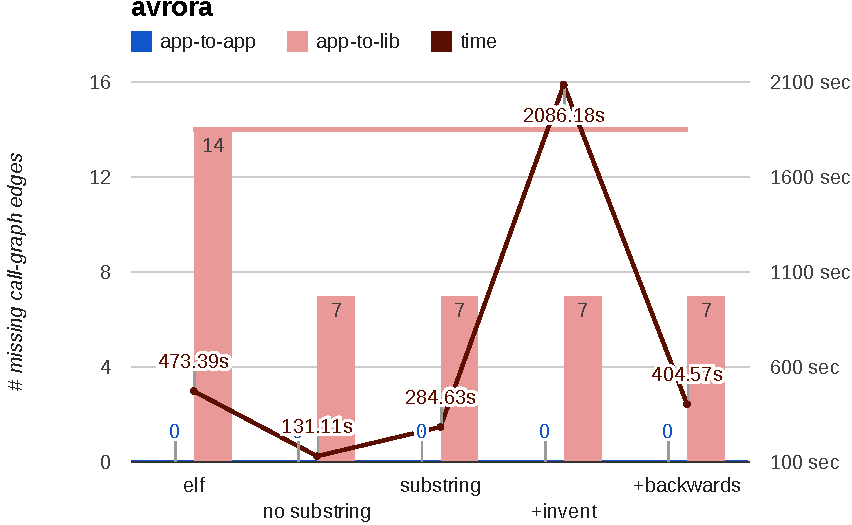
\includegraphics[width=\textwidth,height=0.2\textheight]{%
      figures/reflection/avrora-plain.pdf}
  \end{subfigure}
  ~
  \begin{subfigure}[t]{0.5\textwidth}
    \centering
    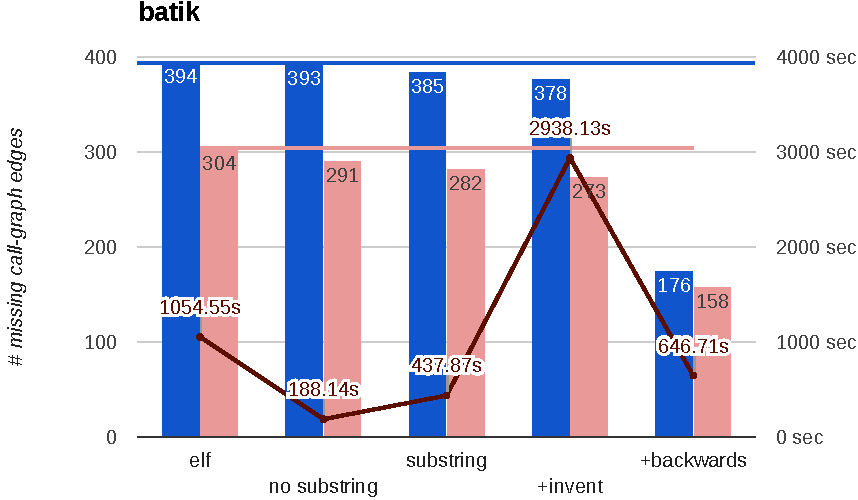
\includegraphics[width=\textwidth,height=0.2\textheight]{%
      figures/reflection/batik-plain.pdf}
  \end{subfigure}
  \\

  % 2nd row
  \begin{subfigure}[t]{0.5\textwidth}
    \centering
    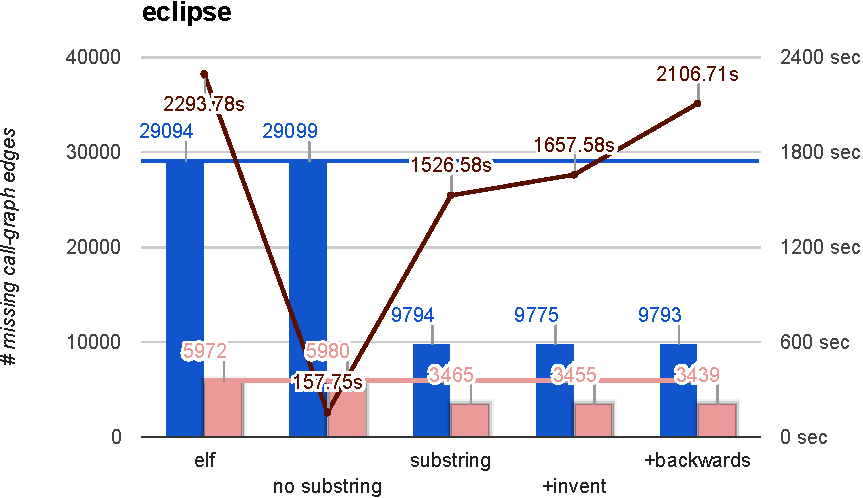
\includegraphics[width=\textwidth,height=0.2\textheight]{%
      figures/reflection/eclipse-plain.pdf}
  \end{subfigure}
  ~
  \begin{subfigure}[t]{0.5\textwidth}
    \centering
    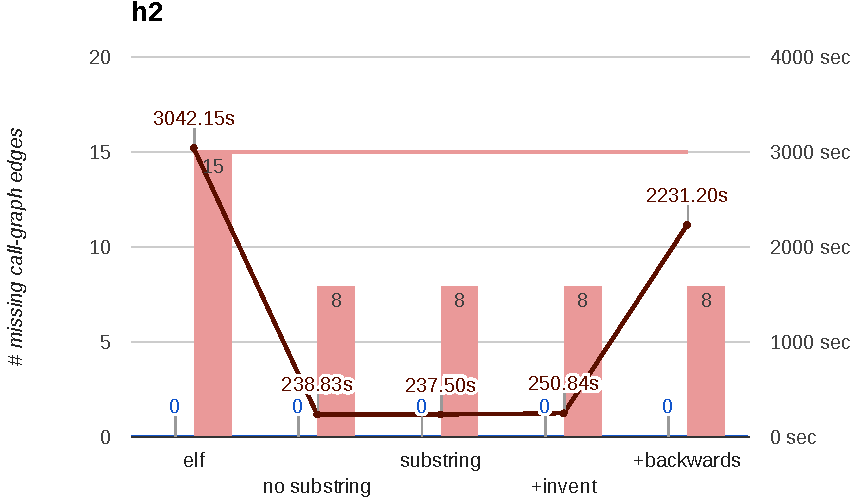
\includegraphics[width=\textwidth,height=0.2\textheight]{%
      figures/reflection/h2-plain.pdf}
  \end{subfigure}
  \\

  % 3rd row
  \begin{subfigure}[t]{0.5\textwidth}
    \centering
    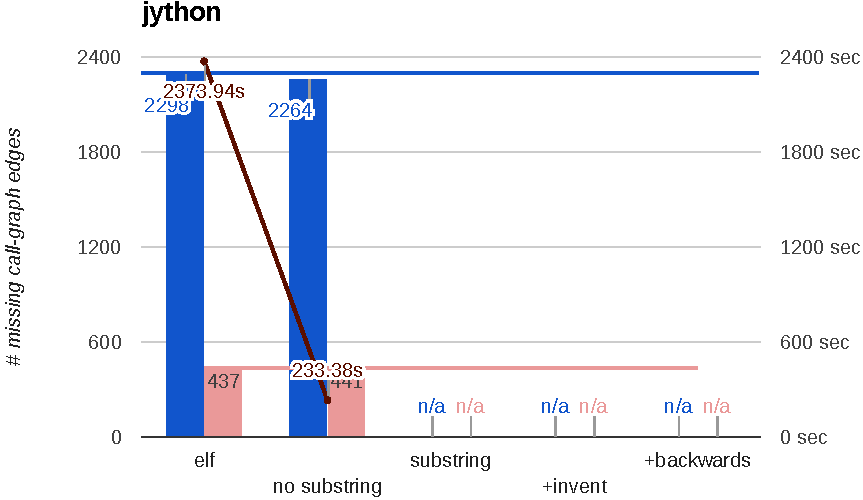
\includegraphics[width=\textwidth,height=0.2\textheight]{%
      figures/reflection/jython-plain.pdf}
  \end{subfigure}
  ~
  \begin{subfigure}[t]{0.5\textwidth}
    \centering
    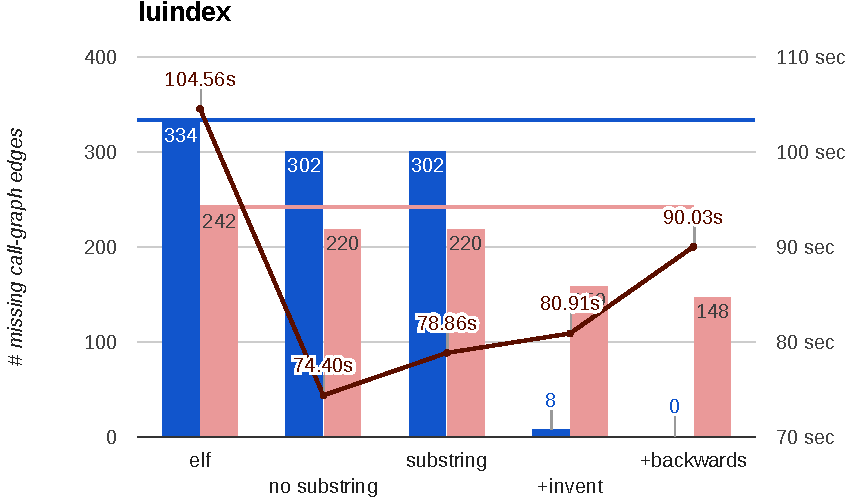
\includegraphics[width=\textwidth,height=0.2\textheight]{%
      figures/reflection/luindex-plain.pdf}
  \end{subfigure}
  \\

  % 4th row
  \begin{subfigure}[t]{0.5\textwidth}
    \centering
    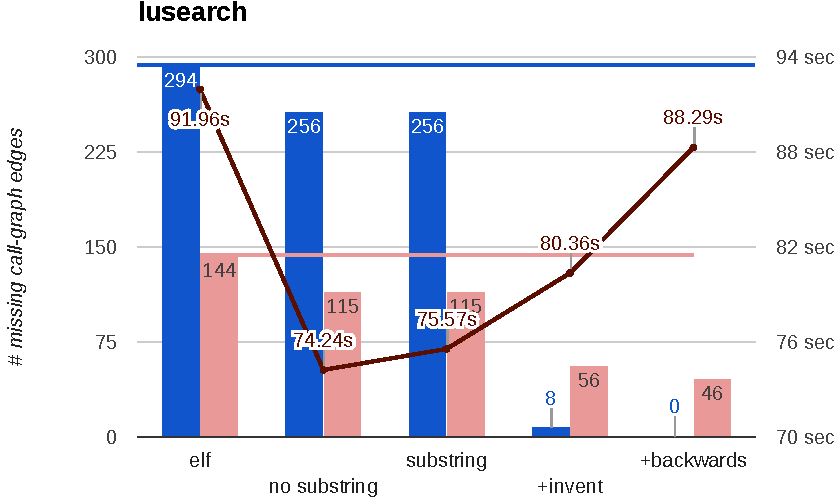
\includegraphics[width=\textwidth,height=0.2\textheight]{%
      figures/reflection/lusearch-plain.pdf}
  \end{subfigure}
  ~
  \begin{subfigure}[t]{0.5\textwidth}
    \centering
    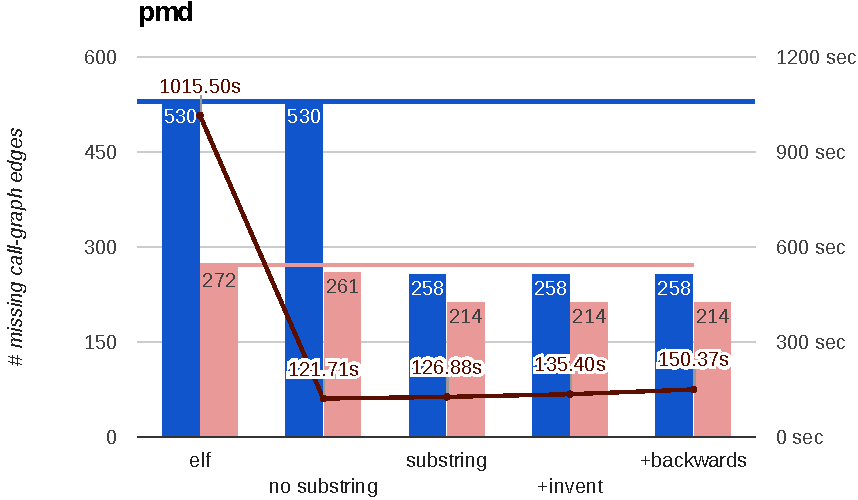
\includegraphics[width=\textwidth,height=0.2\textheight]{%
      figures/reflection/pmd-plain.pdf}
  \end{subfigure}
  \caption[Unsoundness metrics]{%
    Unsoundness metrics (two bars: missing call-graph edges app-to-app
    and app-to-lib) and analysis time (line) over the DaCapo
    benchmarks. \emph{Lower is better for all.} For missing bars
    (``n/a''), the analysis did not terminate in 90mins.}
\end{figure}
\begin{figure}\ContinuedFloat
  % 5th row
  \begin{subfigure}[t]{0.5\textwidth}
    \centering
    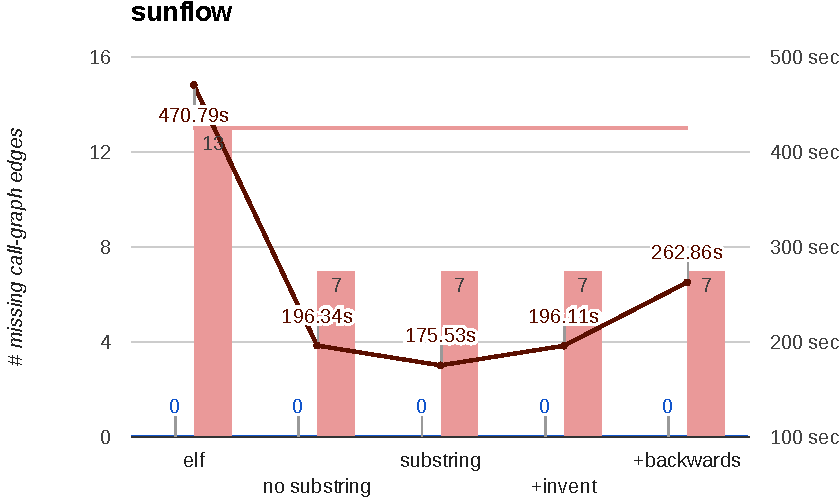
\includegraphics[width=\textwidth,height=0.2\textheight]{%
      figures/reflection/sunflow-plain.pdf}
  \end{subfigure}
  ~
  \begin{subfigure}[t]{0.5\textwidth}
    \centering
    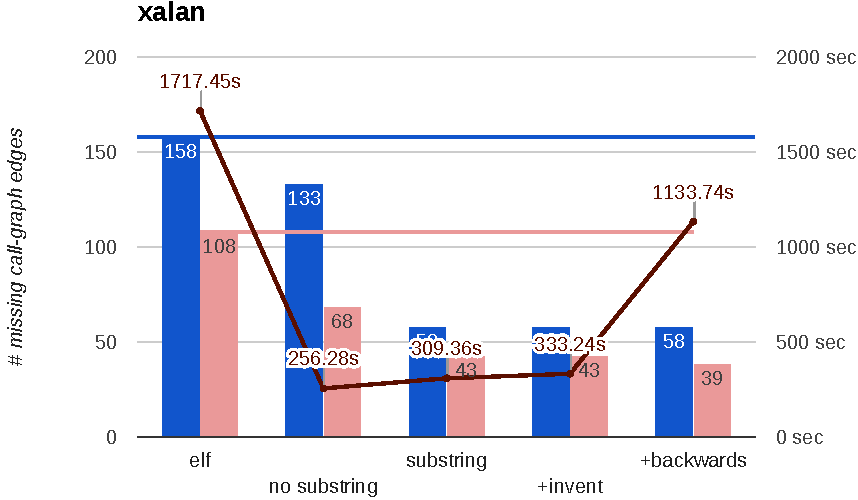
\includegraphics[width=\textwidth,height=0.2\textheight]{%
      figures/reflection/xalan-plain.pdf}
  \end{subfigure}


  % lusearch and sunflow could be left out

  \caption{Unsoundness metrics (cont.)}
  \label{reflection/fig:dacapo-bach}
\end{figure}

% \begin{figure}[t]
%   % \vspace{-1.5cm}
%   % \small
%   \scriptsize
%   \renewcommand{\tabcolsep}{1mm}
%   % \hspace*{-6mm}
%   \centering
%   \begin{tabular}{rrrrrrrrrrr}
%     \toprule
%     \textbf{Total Edges}
%     & \multicolumn{10}{c}{Benchmarks} \\
%     \cmidrule{2-11}
%     Setting & \centercell{avrora} & \centercell{batik} & \centercell{eclipse} & \centercell{h2} & \centercell{jython} & \centercell{luindex} & \centercell{lusearch} & \centercell{pmd} & \centercell{sunflow} & \centercell{xalan} \\
%     \midrule
%     elf & 19355 & 31602 & 10191 & 38252 & 19709 & 4547 & 4209 & 8544 & 4223 & 35918 \\
%     no substring & 19379 & 31708 & 9032 & 35538 & 20537 & 4676 & 4352 & 8592 & 4251 & 35221 \\
%     substring & 20591 & 35314 & 115967 & 38107 & n/a & 4682 & 4362 & 9533 & 4285 & 45160 \\
%     +invent & 26586 & 47303 & 116635 & 38162 & n/a & 5773 & 5266 & 9557 & 4319 & 45343 \\
%     +backwards & 20677 & 37013 & 117576 & 43952 & n/a & 6115 & 5587 & 9577 & 4407 & 63746 \\
%     \midrule
%     dynamic & 4165 & 8329 & 40026 & 4901 & 13583 & 3027 & 1845 & 4874 & 2215 & 6128 \\
%     \bottomrule
%   \end{tabular}
%   \footnotesize
%   \caption{Total static and dynamic call-graph edges for the DaCapo 9.12-Bach
%     benchmarks. These include only \emph{application-to-application}
%     and \emph{application-to-library} edges.}
%   \label{reflection/fig:total_static}
% \end{figure}

\begin{figure}[h]
  \renewcommand{\tabcolsep}{1.5mm}
  \centering
  \begin{tabular}{lr@{ \quad }rrrrr}
    \toprule
    \textbf{Total Edges} & & \multicolumn{5}{c}{Settings} \\
    \cmidrule(l){3-7}
    Benchmark & \emph{dynamic} & elf & no substring 
              & substring & +invent & +backwards
    \\
    \midrule
    avrora & 4165 & 19355 & 19379 & 20591 & 26586 & 20677 \\
    batik & 8329 & 31602 & 31708 & 35314 & 47303 & 37013 \\
    eclipse & 40026 & 10191 & 9032 & 115967 & 116635 & 117576 \\
    h2 & 4901 & 38252 & 35538 & 38107 & 38162 & 43952 \\
    jython & 13583 & 19709 & 20537 & n/a & n/a & n/a \\
    luindex & 3027 & 4547 & 4676 & 4682 & 5773 & 6115 \\
    lusearch & 1845 & 4209 & 4352 & 4362 & 5266 & 5587 \\
    pmd & 4874 & 8544 & 8592 & 9533 & 9557 & 9577 \\
    sunflow & 2215 & 4223 & 4251 & 4285 & 4319 & 4407 \\
    xalan & 6128 & 35918 & 35221 & 45160 & 45343 & 63746 \\
    \bottomrule
  \end{tabular}
  \caption[Total static and dynamic call-graph edges -- DaCapo
  9.12-Bach benchmarks]{Total static and dynamic call-graph edges for
    the DaCapo 9.12-Bach benchmarks. These include only
    \emph{application-to-application} and
    \emph{application-to-library} edges.}
  \label{reflection/fig:total_static}
\end{figure}


Figure~\ref{reflection/fig:dacapo-bach} plots the results of our experiments,
combining both analysis time and empirical unsoundness (in call-graph
edges). 
%We compare our techniques to the \textsc{Elf} system
%\cite{ecoop/LiTSX14}, which also attempts to improve reflection
%analysis for Java. 
% Missing bars labeled ``n/a'' correspond to analyses
% that did not terminate in 90mins (5400sec). 
Each chart plots the
missing dynamic call-graph edges that are not discovered by the
corresponding static analysis. We use separate bars for the
\emph{application-to-application} and \emph{application-to-library}
edges.

% Library-to-library edges are also computed but they are not
% comparable in static vs. dynamic analysis due to native calls.
We consider only call-graph edges originating from application code,
since library classes contain a fair amount of non-analyzable native
methods.\footnote{Call-graph edges from the library are still fully
  statically analyzed, thus our experiments demonstrate scalability
  relative to large libraries. We just do not report
  library-originating edges (though they are computed within the time
  reported) since these only cloud the picture, due to native
  code. There is no easy way to compare library-to-library results to
  dynamic edges without manual filtering, which raises validity
  questions.}
% which \textsc{Doop} cannot analyze at all.
%
We also filter out some missing edges (i.e., consider them implicitly
covered), which involve the following methods:
\begin{itemize}
%[$\cdot$]
\item \emph{Class Initializers.}  \textsc{Doop} only models
%  Due to \textsc{Doop}'s modeling of
%  class initialization, no call-graph edges to and from \code{<clinit>}
%  methods are recorded. Instead, the analysis tracks down only
  \emph{which} subset of classes get initialized (without any
  information about where the initializer gets called from). We filter
  out edges to class initializer methods (i.e., \code{<clinit>}), if
  static analysis indicates that the class has been initialized.
\item \emph{Native.} Native code cannot be analyzed. However, some
  library reflection calls are wrappers for native methods (e.g.,
  \code{forName()} and \code{forName0()}). Edges to these methods are,
  thus, completely extraneous due to our special modeling
  of their effect.
\item \emph{Class Loader.} Method \code{loadClass()} is invoked by the
  VM when a class needs to be loaded and \code{checkPackageAccess()} is
  invoked right after loading.
  %% checkPackageAccess() is private and called automatically by the
  %% VM.
\item \emph{Synthetic.} Edges involving dynamically generated classes
  are impossible to obtain by reflection analysis alone, so we eliminate
  such instances.
\end{itemize}

%
% We filter out edges to implicit methods (static initializers,
% \code{loadClass()}) that are not statically modeled.

We show five techniques:

\begin{asparaenum}
\item \emph{Elf.} This is the \textsc{Elf} reflection analysis
  \cite{ecoop/LiTSX14}, which also attempts to improve reflection
  analysis for Java. 
%It serves as a baseline for the evaluation of the
%  four settings of our own analysis.
\item \emph{No substring.} Our reflection analysis, with 
  engineering enhancements over the original \textsc{Doop} framework,
  but no analysis of partial strings or their flow.
\item \emph{Substring.} The analysis integrates the substring and
  substring flow analysis of Section~\ref{reflection/sec:strings}.
\item \emph{+Invent.} This analysis integrates substring analysis as well as the
  object invention technique of Section~\ref{reflection/sec:invention}.
\item \emph{+Backwards.}\footnote{The \emph{+Backwards} and
    \emph{+Invent} techniques %are not comparable: they
    are both additions to the substring analysis, but neither includes
    the other.} This analysis integrates substring analysis as well as
  the back-propagation technique of
  Section~\ref{reflection/sec:back-propagation}.
\end{asparaenum}


It is important to note that, by design, our techniques
do not enhance the precision of an analysis, only its empirical
soundness.  Thus, the techniques
only find \emph{more} edges: they cover more of the
program. This improvement appears as a reduction in the figures
(``lower is better'') only because the number plotted is the
\emph{difference} in the missing edges compared to the dynamic
analysis.

Our research questions can now be answered:

\begin{description}
\item[RQ1: Do our techniques impact soundness?]
  As can be seen, our techniques substantially increase the soundness
  of the analysis.  In most benchmarks, more than half (to nearly all)
  of the missing \emph{application-to-application} edges are
  recovered by at least one technique. The
  \emph{application-to-library} missing edges also decreased, although
  not as much.  In fact, the \emph{eclipse} benchmark was hardly being
  analyzed in the past, since most of the dynamic call-graph was
  missing.

\item[RQ2: Do the techniques have reasonable running times?]
  Furthermore, although our approach emphasizes empirical soundness,
  it does not sacrifice scalability. All four of our settings are
  faster than \textsc{Elf} for almost all benchmarks. Aside from
  \emph{jython}, for which only the \textsc{Elf} and \emph{no
    substring} techniques are able to terminate before timeout, in
  all other cases \emph{substring} and at least one of \emph{+invent}
  or \emph{+backwards} outperformed \textsc{Elf}, while in 7-of-10
  benchmarks \emph{all} our techniques outperformed \textsc{Elf}.
  This is due to achieving scalability using the threshold techniques
  of Section~\ref{reflection/sec:throttling} instead of by sacrificing some
  empirical soundness, as \textsc{Elf} does. (A major design feature
  of \textsc{Elf} is that it explicitly avoids inferring reflection
  call targets when it cannot fully disambiguate them.)

%  In engineering terms, \textsc{Elf} is not comparable to our
%  approach, since it uses different underlying techniques. In contrast
%  to our emphasis on empirical soundness (e.g., with inter-procedural
%  backward flow of information from casts), \textsc{Elf} explicitly
%  avoids inferring reflection call targets when it cannot fully
%  disambiguate them. This achieves scalability but at the expense of
%  soundness. Instead, our experiments show that empirical soundness
%  can be achieved while our mechanisms of
%  Section~\ref{reflection/sec:throttling} manage to preserve scalability.

\item[RQ3: Do the techniques sacrifice precision?]
  For completeness, we also show a sanity-checking metric over
  our analyses. Empirical soundness could
  increase by computing a vastly imprecise call-graph. This is not the
  case for our techniques. Figure~\ref{reflection/fig:total_static} lists the
  total static and dynamic edges being computed. On average,
  \emph{+backwards} computes the most static edges (about $4.5$ times
  the number of dynamic edges). On the lower end of the spectrum lies
  \emph{no substring}, with a minimum of $3.4$ times the number of
  dynamic edges being computed.

\end{description}

% \item For 5-of-9 of the DaCapo 2006-10-MR2 benchmarks and for 3-of-9
%   or the DaCapo 9.12-Bach, there is no benefit to be gained by
%   advanced reflection analysis, because, even with baseline
%   techniques, our technique eliminates nearly all unsoundness.
%\item The combined techniques typically achieve quite high empirical
%  soundness.  For all 9 benchmarks from DaCapo 2006-10-MR2 and for
%  8-of-9 benchmarks of DaCapo 9.12-Bach, the recall of dynamic edges
%  for the most-sound technique is over 90\%. For 7-of-9 of the DaCapo
%  2006-10-MR2 and for 5-of-9 of DaCapo 9.12-Bach, the metric is at
%  over 97.5\%. The lowest recall (by at least 20\%) is exhibited by
%  the \emph{eclipse} benchmark, at 67\%. \emph{Eclipse}, however,
%  greatly benefits from our techniques: without substring analysis,
%  its recall drops to just 12\%. More representative benefits are
%  those of \emph{batik} and \emph{pmd v.4.2.5}, for which
%  techniques such as substring analysis and back-propagation lead to
%  discovering a total of over 300 extra real call-graph edges. (The
%  analysis did not terminate with the object invention technique for
%  \emph{batik}.)

% \item The run-time overhead of our analysis techniques ranges from the
%   un-noticeable to the substantial. Substring analysis typically
%   incurs a modest overhead (under 20\% for 14 of the 18 benchmarks)
%   but on occasion multiplies analysis times by large factors. The
%   eclipse benchmark is an extreme case, with analysis time increasing
%   tenfold when substring analysis is performed. However, as we saw
%   above, static analysis for eclipse misses most of the program's
%   behavior without substring analysis. The other two techniques
%   consistently add a 10-30\% overhead each, but with rare extreme
%   outliers, such as a sixfold overhead for back-propagation in the
%   case of \emph{xalan v.2.7.1}.

%\item Substring analysis yields the largest single improvement in
%  empirical soundness. Its recall increase is significant in 7 of the
%  18 benchmarks. Object invention makes a difference over that in 2
%  more benchmarks, and back-propagation improves (over substring
%  analysis) in 6 benchmarks. We do not plot the results of combining
%  object invention and back-propagation because for these benchmarks
%  (and for our current settings of parameters $c$ and $d$ from
%  Section~\ref{reflection/sec:throttling}) they hardly show a difference over
%  back-propagation alone, in either execution time or empirical
%  soundness.

%\item In terms of absolute numbers, each analysis technique typically
%  leads to discovering several tens of missing call-graph edges.

% \end{asparaenum}

%An interesting overall question is which of our techniques an analysis
%user should choose. As in most tunable analyses, 

In pragmatic terms, a user of our analysis should use flags to pick
the technique that yields more soundness without sacrificing
scalability, for the given input program. This is a familiar
approach---e.g., it also applies to picking the exact flavor and depth
of context-sensitivity.

%In summary, our techniques offer useful tradeoffs of soundness
%and scalability. They are  effective at improving our main
%soundness metric (recall of dynamic call-graph edges), and the cost is
%typically quite manageable. 

%Some outliers, in terms of extreme cost
%or extreme recall improvement are worthy of further study.


\section{Related Work}
\label{reflection/sec:related}

The traditional handling of reflection in static analysis has been
through integration of user input or dynamic information.  The
Tamiflex tool~\cite{icse/BoddenSSOM11} exemplifies the state of the
art. The tool observes the reflective calls in an actual execution of
the program and rewrites the original code to produce a version
without reflection calls. Instead, all original reflection calls
become calls that perform identically to the observed execution. This
is a practical approach, but results in a blend of dynamic and static
analysis.
% Clearly, the greatest motivation for
%static analysis is to capture all possible program behaviors. 
It is unrealistic to expect that uses of reflection will always yield
the same results in different dynamic executions---or there would be
little reason to have the reflection (as opposed to static code) in
the first place. Our approach attempts to restore the benefits of
static analysis, with reasonable empirical soundness.

An alternative approach is that of Hirzel et
al.~\cite{ecoop/HirzelDH04,toplas/HirzelDDH07}, where an online
pointer analysis is used to deal with reflection and dynamic loading
by monitoring their run-time occurrence, recording their results, and
running the analysis again, incrementally. This approach is quite
interesting when applicable. However, it is not applicable in many
static analysis settings. Maintaining and running a precise static
analysis during program run time is often not realistic (e.g., for
expensive context-sensitive analyses). Furthermore, the approach does
not offer the off-line soundness guarantees one may expect from static
analysis: it is not possible to ask questions regarding all methods
that may ever be called via reflection, only the ones that have been
called so far.

Interesting work on static treatments of reflection is often in the
context of dynamic languages, where resolving reflective invocations
is a necessity.  Furr et al.~\cite{oopsla/FurrAF09} offer an analysis
of how dynamic features are used in the Ruby language. Their
observations are similar to ours: dynamic features (reflection in our
case) are often used either with sets of constant arguments (in order
to avoid writing verbose, formulaic code), or with known
prefixes/suffixes (e.g., to re-locate within the file system).

Madsen et al.~\cite{sigsoft/MadsenLF13} employ a use-based analysis
technique in the context of Javascript. When objects are retrieved
from unknown code (typically libraries) the analysis infers the
object's properties from the way it is used in the client. In
principle, this is a similar approach to our use-based techniques
(both object invention and back-propagation) although the technical
specifics differ. The conceptual precursor to both approaches is the
work on reflection by Livshits et
al.~\cite{aplas/LivshitsWL05,livshits:thesis}, which has been
extensively discussed and contrasted throughout this chapter (see
Sections~\ref{reflection/sec:model}, and \ref{reflection/sec:use-based}).

Advanced techniques for string analysis have been presented by
Christensen et al.~\cite{sas/ChristensenMS03}. They analyze complex
string expressions and abstract them via a context-free grammar that
is then widened to a regular language. The regular approximations
produced by this approach are richer than the prefix and suffix
matching of our substring analysis, and can thus better approximate
the possible values of arbitrary string expressions. Reflection is one
of their examples but they only apply it to small benchmarks.

\citeauthor{ecoop/AliL12}~\cite{ecoop/AliL12,ecoop/AliL13} offer
comparisons of dynamic and static call-graph edge metrics.  They
discover hundreds of missing edges in several of the DaCapo
2006-10-MR2 benchmarks.  However, their experiments do not integrate
the vastly improved support for reflection (e.g., modeling of
\javasignature{Object.getClass}) offered by \textsc{Elf} or our
current work.

%were performed
%before numerous engineering improvements in the \textsc{Doop}
%framework. 
%These improvements handle many common API calls, such as
%\javasignature{Object.getClass}.
%Furthermore, some benchmarks could not be run with reflection enabled
%due to scalability issues. Therefore, o
%%SPACE
%Our experiments are substantially more representative in regards to
%the actual empirical soundness of a joint reflection and pointer
%analysis.  
Stancu et al.~\cite{pppj/StancuWBLF14} empirically
%present an empirical study that 
compare profiling data with a points-to static analysis.
%,but do not support reflection. 
However, they target only the most reflection-light benchmarks of the
DaCapo 9.12-Bach suite (\emph{avrora, luindex, and lusearch}), and
patch the code to avoid reflection entirely.

%Some of the most closely related work to ours is the Li et
%al. work~\cite{ecoop/LiTSX14}, discussed earlier. Li et al. also
%improve on the engineering aspects of reflection handling in the
%\textsc{Doop} framework, as well as employ a back-propagation
%technique. The work is concurrent to ours and we have only been able
%to obtain a preprint at the time of this writing. Nevertheless, the
%differences of the two approaches seem quite clear, as also discussed
%in Section~\ref{reflection/sec:back-propagation}. Furthermore, the Li et al.
%technique does not employ substring matching or substring flow
%analysis and does not emphasize empirical soundness. Instead it
%eagerly under-approximates many more reflective calls and resolves
%such calls only when forward and backward reflection analysis
%information agrees. A valuable aspect of the Li et al. work is a
%detailed study of how reflection is used in practical programs.


\section{Conclusions}

%Reflection is of key importance, yet very hard to handle in static
%analysis.  We presented powerful techniques that elegantly extend
%declarative reasoning over reflection calls and inter-procedural
%object flow.


Highly dynamic features, such as reflection and dynamic loading, are
the bane of static analysis. These features are not only hard to
analyze well, but also ubiquitous in practice, thus limiting the
practical impact of static analysis. We presented techniques for
static reflection handling in Java program analysis. Our techniques
build on top of state-of-the-art handling of reflection in Java, by
elegantly extending declarative reasoning over reflection calls and
inter-procedural object flow. Our main emphasis has been in achieving
higher empirical soundness, i.e., in having the static analysis truly
model observed dynamic behaviors. Although full soundness is
infeasible for a realistic analysis, it is possible to produce
general techniques that enhance the ability to analyze reflection calls.

Although our techniques improve on the problem of handling reflection,
further work is necessary to achieve 
good scalability and empirical
soundness for complex programs.
% and sophisticated analysis algorithms. 
Furthermore, our work has not addressed another major and
commonly used dynamic feature: dynamic loading. Continued work will
hopefully make such language features a lot more feasible to analyze
statically.

\begin{comment}
Our treatment of reflection is
probably not the definitive solution to this problem of never-ending
complexity. Nevertheless, we believe it is an important step and it is
highly interesting (probably surprising to most experts) that
empirical soundness can be achieved without any external input for
widely used benchmark programs of significant complexity.

Other standard optimizations included allocating all reified fields,
objects, and constructors without context: they are immutable
objects. This was already done for reified classes.

The second challenge was to improve the scalability of
context-sensitive analyses under reflection. The natural first move
was to remove context-sensitivity from reflective method invocations
and reflective object allocations. Even the old code wasn't too good
at this: it didn't use the standard macros for creating new hcontexts
at reflective allocation sites, and at reflective call sites
(reflective virtual and reflective special) it just propagated the
context of the caller method. Instead, I now create a unique context
object (different from normal ones) and use that. This turns out to
lose virtually no precision (in any client-level metric), and in many
cases slightly *increased* precision (because even though it's just a
single calling context for all reflective calls, it cannot be confused
with normal calls to the same method). If one *wants*
context-sensitive reflection, then there is a preprocessor flag to
enable it (with the right macros for context creation, this time).


-tracking the flow of strings through StringBuffer and StringBuilder
objects In fact, this can be done in two modes: either by treating all
string factories as one object, or by distinguishing them.

-treating System and Application classes differently: it makes little
sense to access System classes via reflection. Their names, packages,
etc. are known to application code and to other system code. In
general, we care much more about application classes accessed via
reflection (which is a legitimate functionality for ultra-general
system code, as well as for other application code that tries or
adapts to configuration changes).

-tracking so many string constants (class/method/field names and
substrings of those) is extremely costly. Therefore there is the
ability to merge all of them into one constant (or, really, 3
representatives, since they are distinguished by type: one for all
class-name strings, one for all method-name strings, one for all
field-name strings). This restores scalability of the string object
var-points-to logic but risks losing scalability due to reflective
object flow tracking, in benchmarks that do use reflection seriously.

\end{comment}


%%% Local Variables:
%%% mode: latex
%%% TeX-master: "../thesis"
%%% End:
